\documentclass[a4paper,twoside]{report}
\usepackage[T1]{fontenc}
\usepackage{fullpage}
\usepackage{graphicx}
\usepackage{pslatex}

%\newcommand{\postscript}[2]{\vskip 0.5cm \setlength{\epsfxsize}{#2\hsize}\centerline{\epsfbox{#1}}}

\graphicspath{{figures/}}  

\begin{document}

\title{\vskip 5cm
  {\huge SynDEx v6 TUTORIAL}\\
}
\author{
       \large \sl \bf  Nicolas Dos Santos, Christophe Macabiau, Yves Sorel \\
}

\maketitle


\cleardoublepage
\tableofcontents

\cleardoublepage
\chapter*{Introduction}
\addcontentsline{toc}{chapter}{Introduction}
\markboth{\uppercase{Introduction}}{Introduction}

The examples presented in this document are located in the directory
\textbf{``syndex-6.6.0/examples/tutorial''}.\\ The example 6 is located in the
directory \textbf{``syndex-6.6.0/examples/tutorial/example6''.}

\medskip

\subsubsection{In the example 1 (algorithm, architecture and adequation):}
\begin{itemize}
\item We create a \textbf{sensor} definition, an \textbf{actuator} definition,
and an \textbf{function} definition. Then, we create an algorithm and define
it as \textbf{main}. Finally, we create in the main algorithm two
\textit{references} to the sensor definition, three references to the actuator
definition, and one reference to the function definition, and we create \textit{data
dependencies} between these references by connecting their ports ;

\item We create four different architectures: 
\begin{itemize}
\item an architecture with one \textbf{operator},
\item an architecture with two \textbf{operators} and a communication media of
type \textbf{SAM Point-to-Point},
\item an architecture with three \textbf{operators} and a communication media
of type \textbf{SAM Multipoint},
\item an architecture with three \textbf{operators} and a communication media
of type \textbf{RAM} ;
\end{itemize}

\item We create \textbf{constraints} on the third architecture,

\item We perform the \textbf{adequation} of the main algorithm onto the third
architecture defined as main, without constraints and then with constraints.
\end{itemize}

\subsubsection{In the example 2 (hierarchy in algorithm):}
\begin{itemize}
\item We create a function definition and inside this function we create a
reference to another operation ; in that way this definition is defined by 
\textit{hierarchy}. Then,
we create an algorithm and define it as \textbf{main}. Finally, we create in
the main algorithm one reference to the hierarchical function ;

\item We create \textbf{parameters names} for an operation, and assign values
to these parameters.

\end{itemize}

\subsubsection{In the example 3 (delay and constant in algorithm):}
\begin{itemize}
\item We create a \textbf{delay}, and a \textbf{constant} definitions,

\item We create a main algorithm by referencing a \textbf{delay},
a \textbf{sensor}, an \textbf{actuator}, an \textbf{function}, and a
\textbf{constant}, and by connecting them.

\end{itemize}

\subsubsection{In the example 4 (repetition and library in algorithm):}
\begin{itemize}
\item We create two algorithms which repeat an operation:
\begin{itemize}
\item a multiplication of a scalar by a vector by repeating a multiplication
function. We create this algorithm without any library, and then with a library ;

\item a multiplication of a vector by a matrix by repeating a multiplication
function.
\end{itemize}

\end{itemize}

\subsubsection{In the example 5 (condition and nested condition in
algorithm):}

We create two conditioned algorithms:
\begin{itemize}
\item an algorithm conditioned by a data dependence the value of which
indicates the operation to be executed,

\item an algorithm conditioned by a data dependence, one operation of which is
in turn conditioned (\textit{nested condition}) by the same data dependence.
\end{itemize}

\subsubsection{In the example 6 (algorithm, architecture, adequation
and code generation):}
\begin{itemize}
\item We create a main algorithm by referencing a \textbf{sensor}, two
\textbf{actuators}, three \textbf{functions}, and a \textbf{constant}, and by
connecting them,

\item We create an architecture with two \textbf{operators} of type
\textbf{U} and a \textbf{communication media} of type \textbf{u/TCP},

\item We perform the adequation,

\item We perform the \textbf{code generation} and we execute the
\textbf{executives} created after compilation.
\end{itemize}

\cleardoublepage
\chapter{Example 1 : algorithm, architecture and adequation}

\section{Creation of the algorithm}
\label{algo_ex1}
\subsection{Creation of a new local definition for a sensor}
\begin{itemize}
\item In the SynDEx principal window, choose in the menu: \textbf{Algorithm / New Local Definition / Sensor} (figure \ref{A_NLD_S}).

\begin{figure}[htbp]
  \begin{center}
        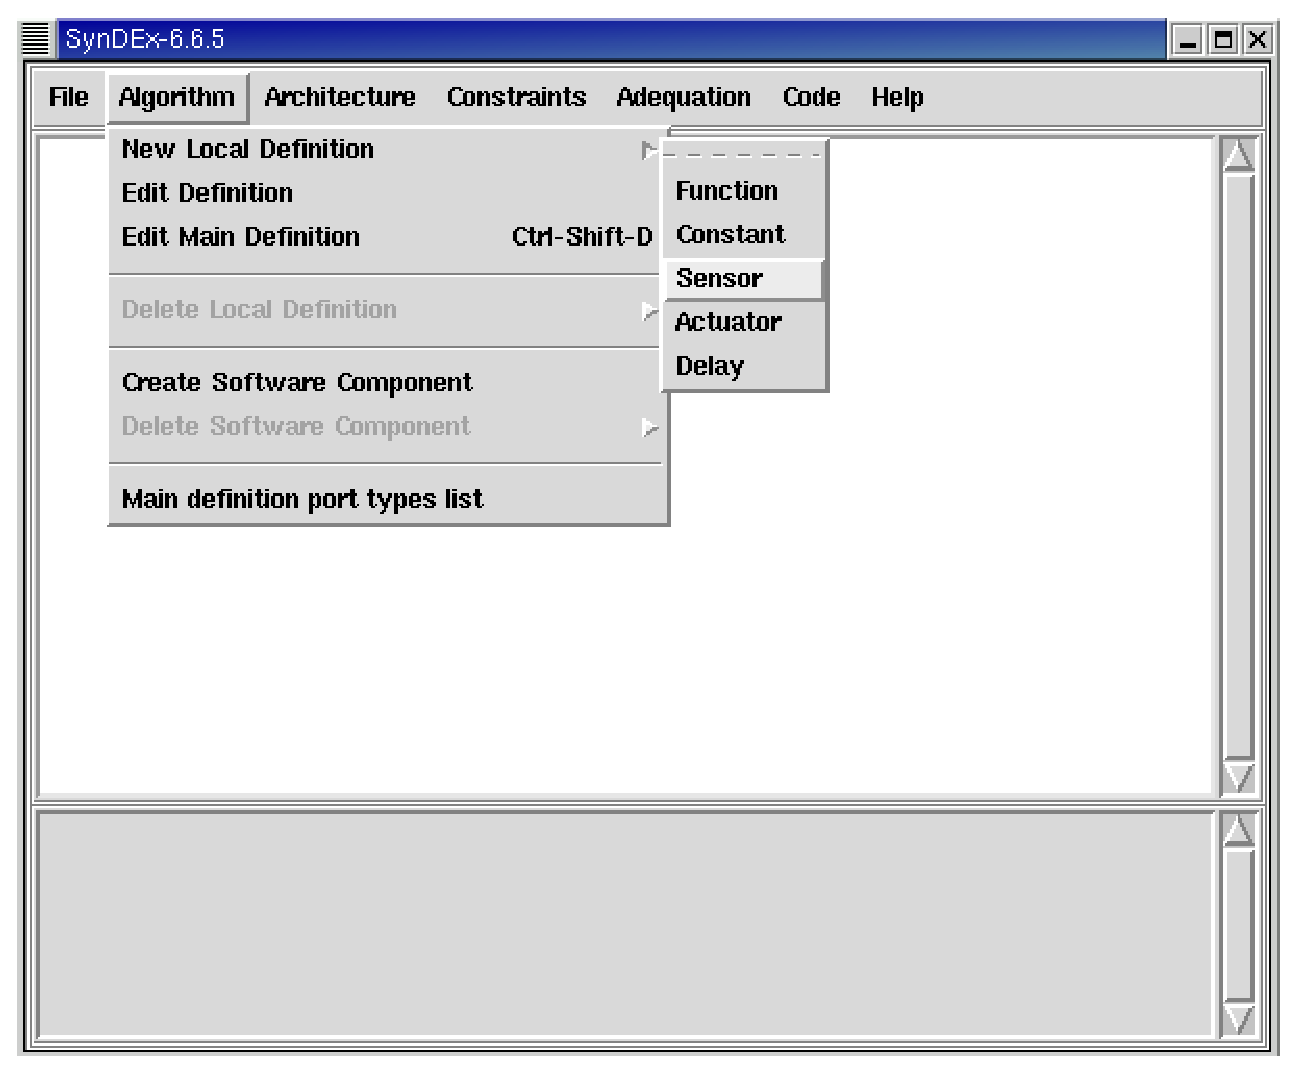
\includegraphics[scale=0.53]{Algorithm_NewLocalDefinition_Sensor.eps}
  \end{center}
  \caption{\textbf{algorithm} $\rightarrow$ \textbf{New Local Definition} $\rightarrow$ \textbf{sensor}}
  \label{A_NLD_S}
\end{figure}

This opens a dialog window (figure \ref{new_definition}) in which you can type
the name and optionally a list of arguments for the sensor. For example type
the name: ``input'', then click OK. This creates a local definition of sensor
named ``input'', and opens the corresponding definition window (figure
\ref{definition_window}).

\begin{figure}[htbp]
  \begin{center}
        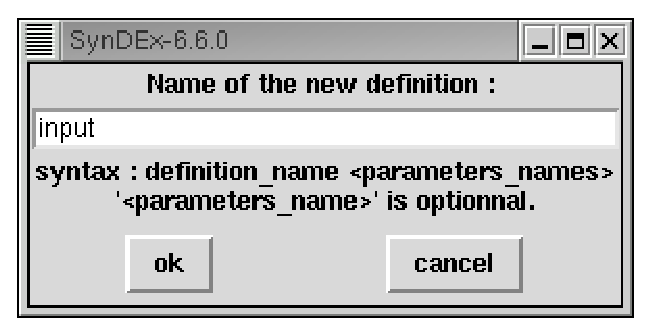
\includegraphics[width=0.45\linewidth]{Name_of_the_new_definition.eps}
  \end{center}
  \caption{Name of the new definition}
  \label{new_definition}
\end{figure}

\begin{figure}[htbp]
  \begin{center}
        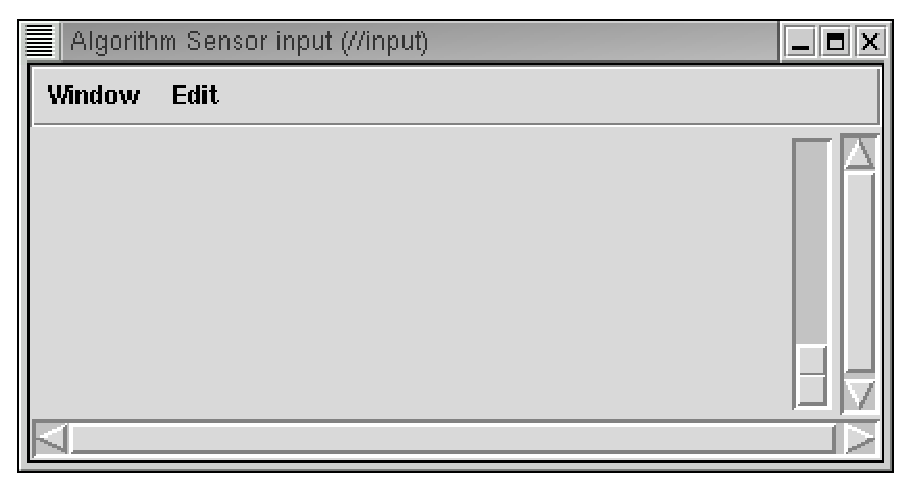
\includegraphics[width=0.5\linewidth]{Definition_window.eps}
  \end{center}
  \caption{Definition window}
  \label{definition_window}
\end{figure}



\item In this definition window, choose in the menu: \textbf{Edit / Create
Port}. This opens a dialog window in which you can type the port name. For
example type the name: ``! int o'', then click OK. This creates the integer
output port named ``o'' (figure \ref{ports}) in the definition window.

\begin{figure}[htbp]
  \begin{center}
        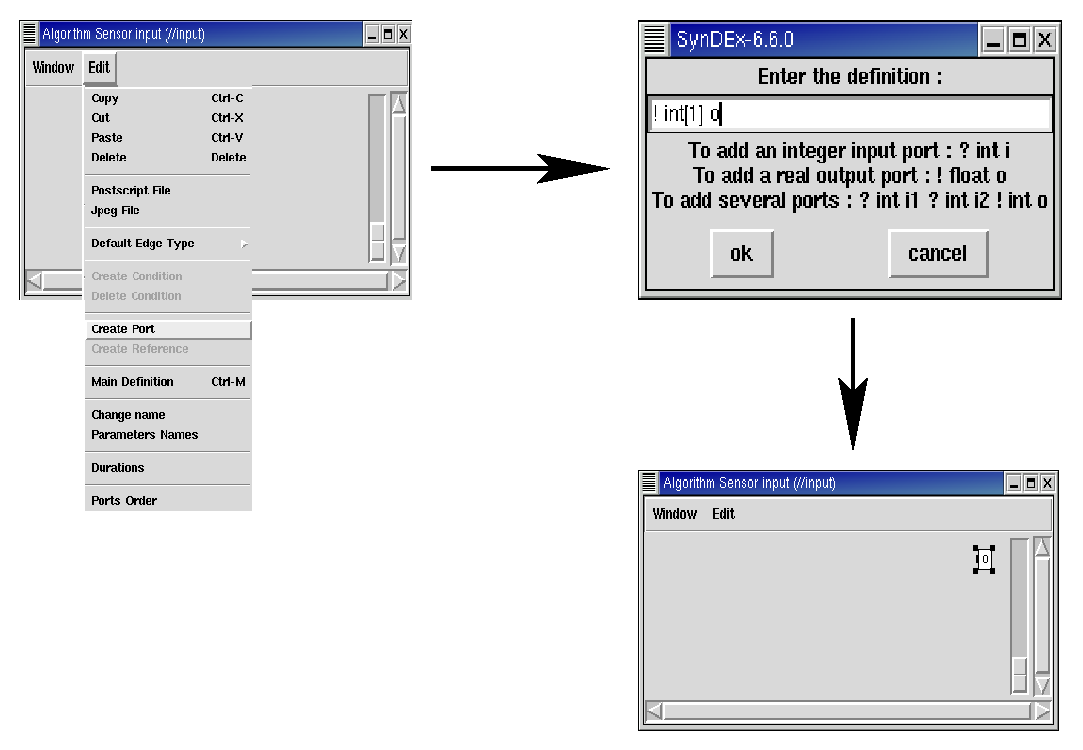
\includegraphics[width=\linewidth]{Edit_CreatePort.eps}
  \end{center}
  \caption{Creation of the ports}
  \label{ports}
\end{figure}

\end{itemize}

\subsection{Creation of a new local definition for an actuator}
\begin{itemize}
\item In the principal window, 

Menu: \textbf{Algorithm / New Local Definition / Actuator} $\rightarrow$
DialogWindow: ``output'', click OK $\rightarrow$ DefinitionWindow

\item In the definition window,

Menu: \textbf{Edit / Create Port}$\rightarrow$ DialogWindow: ``? int i'', click
OK

\end{itemize}

\subsection{Creation of a new local definition for a function}
\begin{itemize}
\item In the principal window, 

Menu: \textbf{Algorithm / New Local Definition / Function} $\rightarrow$
DialogWindow: ``computation'', click OK $\rightarrow$ DefinitionWindow

\item In the definition window,

Menu: \textbf{Edit / Create Port}$\rightarrow$ DialogWindow: ``? int a ?  int b
! int o'', click OK

\end{itemize}

\subsection{Creation of the main algorithm definition}
\begin{itemize}
\item In the principal window, 

Menu: \textbf{Algorithm / New Local Definition / Function} $\rightarrow$
DialogWindow: ``AlgorithmMain'', click OK $\rightarrow$ DefinitionWindow

\item In the definition window, to define this algorithm as the main algorithm,

Menu: \textbf{Edit / Main Definition} ; or the short key CTRL + M

\item In the definition window,
\begin{itemize}
\item to create a reference to the \textbf{sensor} ``input'',

Menu: \textbf{Edit / Create Reference}
$\rightarrow$ DialogWindow: click \textbf{local}, select \textbf{input}
$\rightarrow$ DialogWindow: ``in1 in2'' (figure \ref{in1_in2})

\begin{figure}[htbp]
        \begin{center} 
        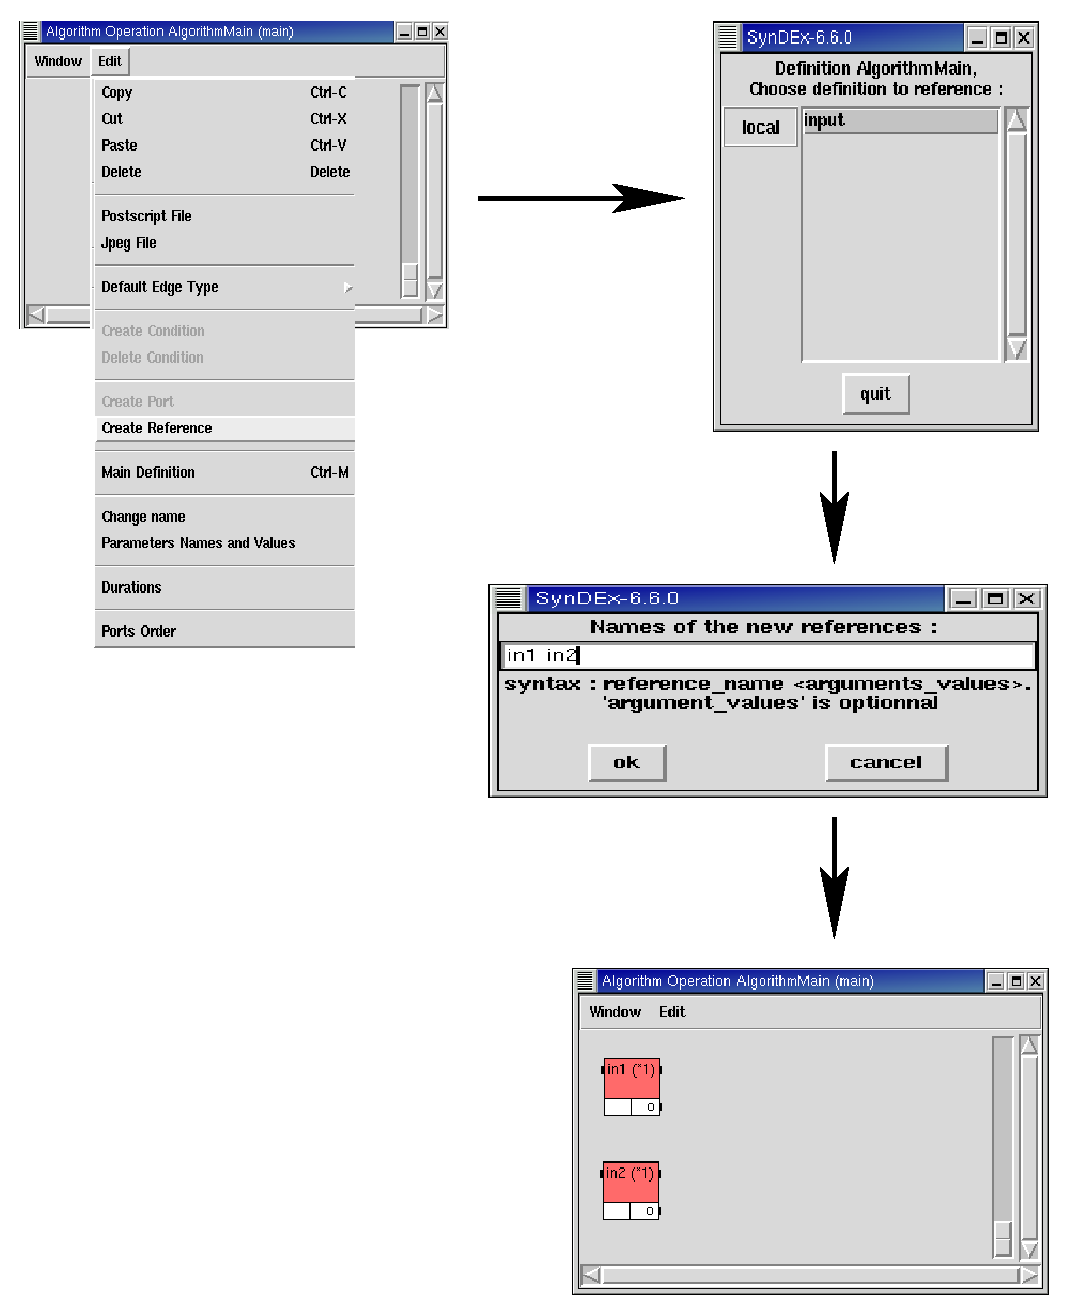
\includegraphics[width=\linewidth]{Edit_CreateReference.eps}
        \end{center}

\caption{\textbf{Edit $\rightarrow$ Create Reference $\rightarrow$ local button
$\rightarrow$ input}}

\label{in1_in2}
\end{figure}

\item to create a reference to the \textbf{actuator} ``output'',

Menu: \textbf{Edit / Create Reference}
$\rightarrow$ DialogWindow: click \textbf{local}, select \textbf{output}
$\rightarrow$ DialogWindow: ``out1 out2 out3''

\item to create a reference to the \textbf{function} ``computation'', 

Menu: \textbf{Edit / Create Reference}
$\rightarrow$ DialogWindow: click \textbf{local}, select \textbf{computation}
$\rightarrow$ DialogWindow: ``calc''

\end{itemize}


\item In the main algorithm window, to create a data dependence between the
``in1'' operation reference and the ``calc'' operation reference, point the
cursor on the output port ``o'' of the ``in1'' operation and click on the
middle button of the mouse (or CTRL+click left button of the mouse) and drag to
the input port ``a'' of the ``calc'' operation. This draws an arrow between the
ports of these operations. After creating the other data dependences, the main
algorithm looks like figure \ref{algo1}.

\end{itemize}

\begin{figure}[htbp]
  \begin{center}
       \includegraphics[scale=0.75]{algorithm_ex1.eps}
  \end{center}
  \caption{Algorithm of the example 1}
  \label{algo1}
\end{figure}


\section{Creation of architecture with one operator}
\label{archi1u_ex1}
\subsection{Creation of a new operator definition}
\label{operator}
\begin{itemize}
\item In the principal window, 

Menu: \textbf{Architecture / New Local Operator Definition}
$\rightarrow$ DialogWindow: ``Uinout'', click OK $\rightarrow$ DefinitionWindow

\item In the definition window (figure \ref{archi}):
\begin{itemize}
\item to add the gates: click \textbf{Modify gates} $\rightarrow$ DialogWindow:
``gate\_type\_1 x''
\item to associate, to each operator of this type, execution durations: click \textbf{Modify
durations} $\rightarrow$ DialogWindow: 

``computation = 2 
 
\hspace{4pt}input = 1 

\hspace{4pt}output = 3''
\end{itemize}

\begin{figure}[htbp]
  \begin{center} 
        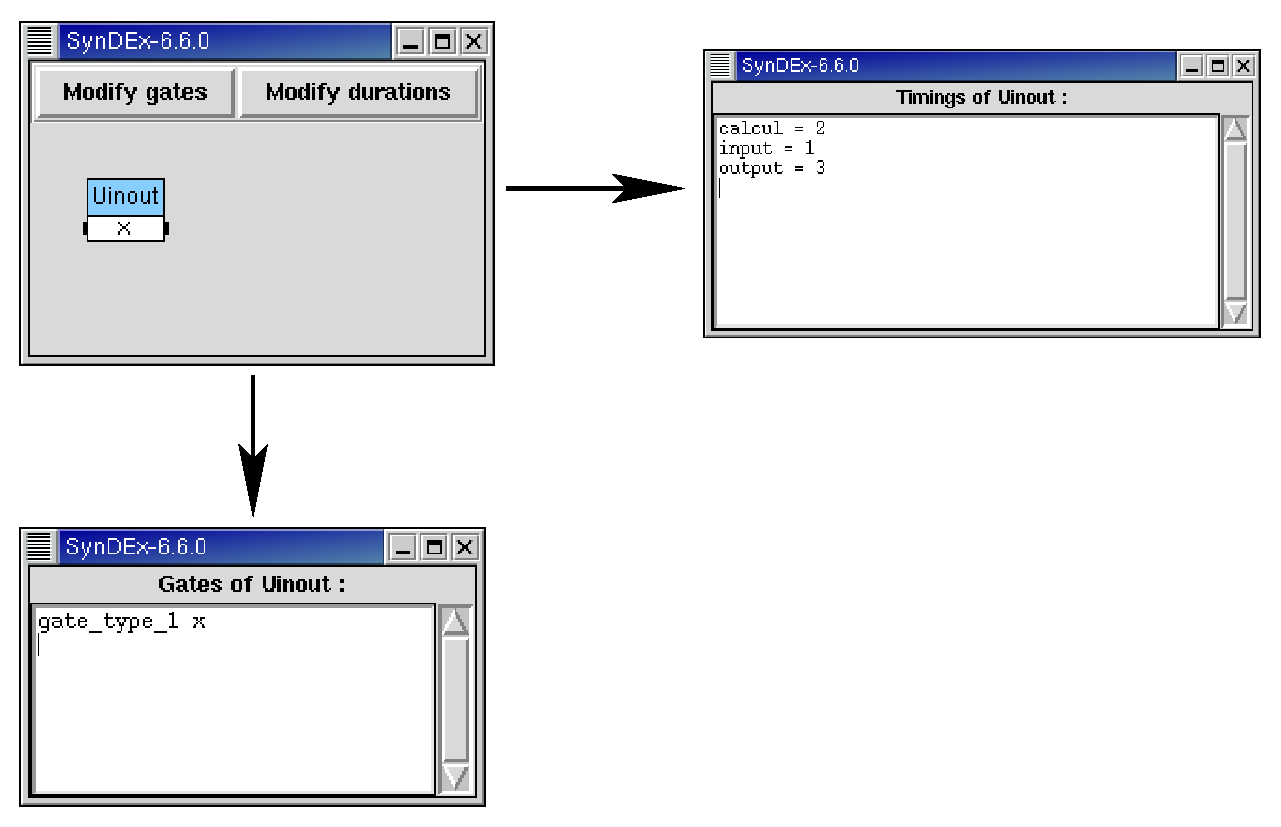
\includegraphics[width=\linewidth]{archi.eps} 
  \end{center}
  \caption{Gates and durations} 
  \label{archi}
\end{figure}

\end{itemize}

\subsection{Creation of the main architecture definition}
\label{main_archi_ex1}
\begin{itemize}
\item In the principal window, 

Menu: \textbf{Architecture / New Local Architecture} $\rightarrow$
DialogWindow ``ArchiOneOperator'' $\rightarrow$ DefinitionWindow (figure \ref{A_NLA}).

\begin{figure}[htbp]
  \begin{center}
       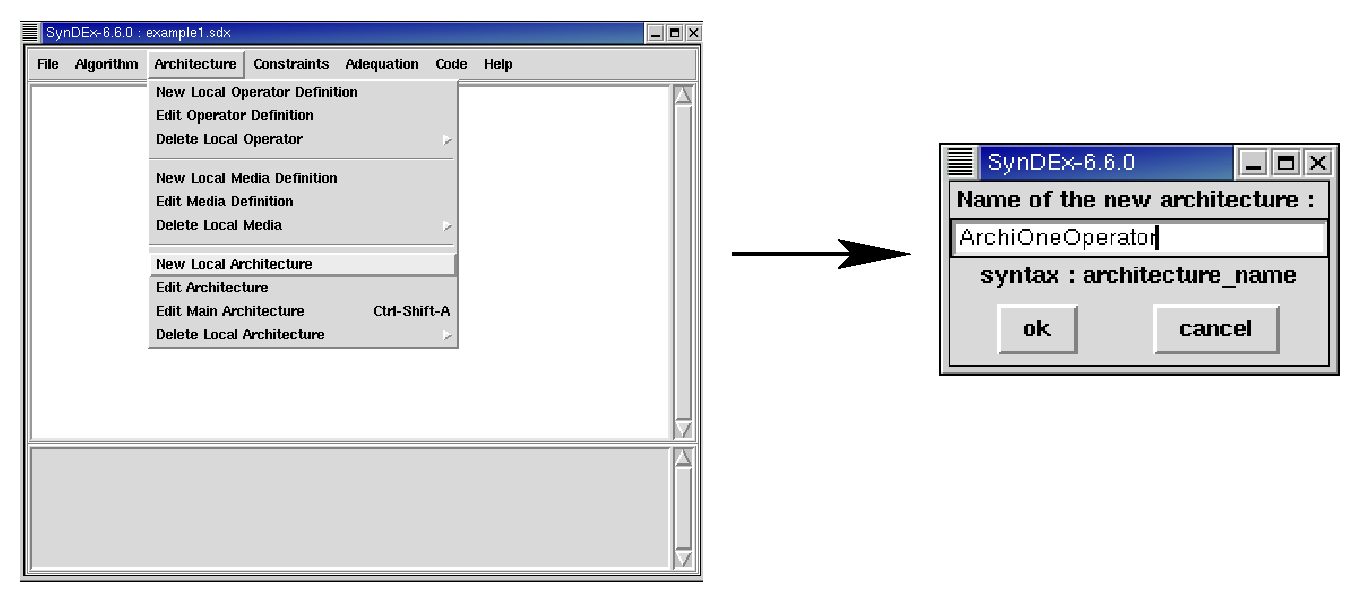
\includegraphics[width=\linewidth]{Architecture_NewLocalArchitecture.eps}
  \end{center}
  \caption{\textbf{Architecture $\rightarrow$ New Local Architecture $\rightarrow$ Name of the new Architecture}}
  \label{A_NLA}
\end{figure}

\item In the definition window, to define this architecture as the main architecture: 

Menu: \textbf{Edit / Main Architecture} ; or the short key CTRL + M.

\item In the main architecture window,

\begin{itemize}
\item to create a reference to the \textbf{operator} `` Uinout'', 

Menu: \textbf{Edit / Create Operator Reference} $\rightarrow$ DialogWindow: click
\textbf{local}, select \textbf{Uinout} $\rightarrow$ DialogWindow: ``u1'' (figure\ref{Uinout})

\begin{figure}[htbp]
  \begin{center} 
        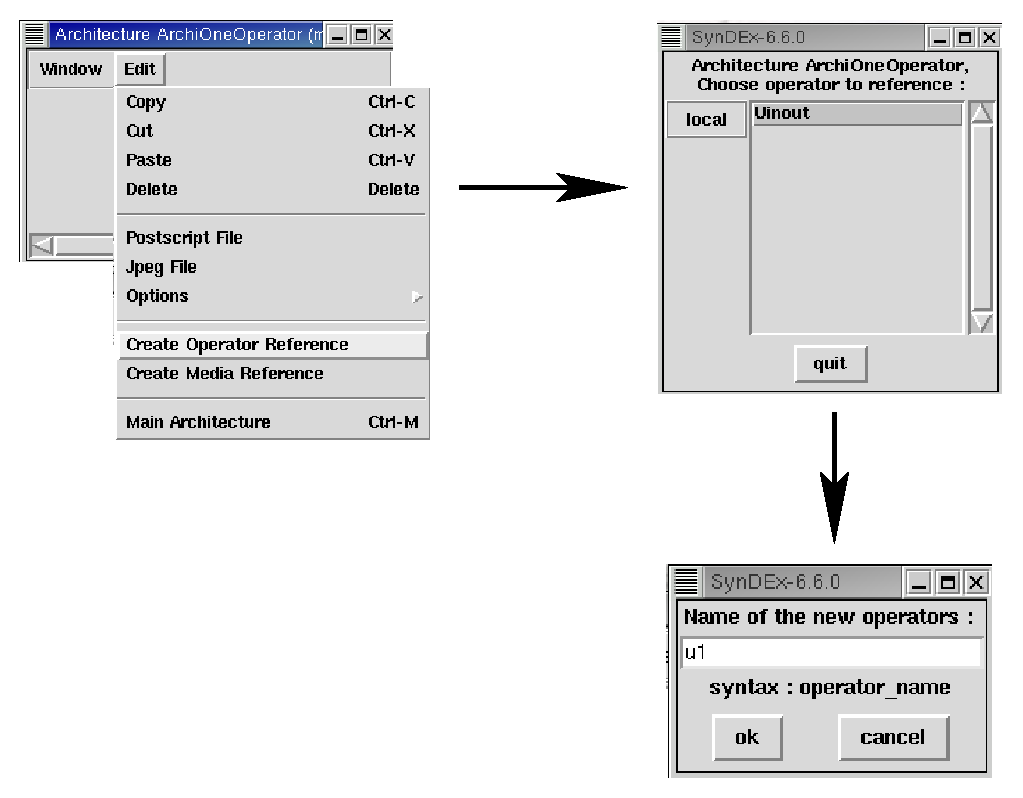
\includegraphics[width=0.92\linewidth]{Edit_CreateOperatorReference.eps} 
  \end{center}
  \caption{\textbf{Edit $\rightarrow$ Create Operator Reference $\rightarrow$ local button $\rightarrow$ Uinout}} 
  \label{Uinout}
\end{figure}

\item to define an operator as main, click on the mouse right button,
and select \textbf{Main Operator}.

\end{itemize}
The architecture looks like the figure \ref{archi1}.
\begin{figure}[htbp]
  \begin{center} 
        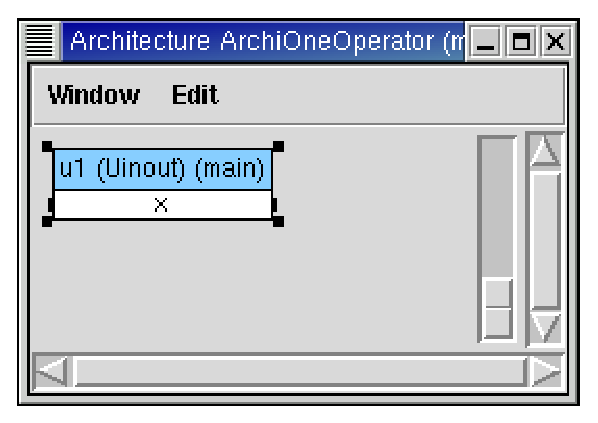
\includegraphics[width=.41\linewidth]{architecture_ex1.eps} 
  \end{center}
  \caption{Architecture of the example 1} 
  \label{archi1}
\end{figure} 

\end{itemize}

\section{Creation of architecture with two operators and a media of communication (Sam
        Point to Point)}
\subsection{Creation of new operator definitions}
\begin{itemize}
\item In the principal window,

Menu: \textbf{Architecture / New Local Operator Definition} $\rightarrow$
DialogWindow: ``Uin'', click OK $\rightarrow$ DefinitionWindow

\item In the definition window,
\begin{itemize}
\item click \textbf{Modify gates} $\rightarrow$ DialogWindow:

``MediaSamPointToPoint x

\hspace{4pt}MediaSamMultiPoint y

\hspace{4pt}MediaRam z''
\item click \textbf{Modify durations} $\rightarrow$ DialogWindow: 

``computation = 2 
 
\hspace{4pt}input = 2

\hspace{4pt}output = 5''
\end{itemize}

\item In the principal window,

Menu: \textbf{Architecture / New Local Operator Definition} $\rightarrow$
DialogWindow: ``Uout'', click OK $\rightarrow$ DefinitionWindow

\item In the definition window,
\begin{itemize}
\item click \textbf{Modify gates} $\rightarrow$ DialogWindow:

``MediaSamPointToPoint x

\hspace{4pt}MediaSamMultiPoint y

\hspace{4pt}MediaRam z''
\item click \textbf{Modify durations} $\rightarrow$ DialogWindow: 

``computation = 2 
 
\hspace{4pt}input = 5

\hspace{4pt}output = 3''

\end{itemize}
\end{itemize}

\subsection{Creation of a new media definition}

\begin{itemize}
\item In the principal window, 

Menu: \textbf{Architecture / New Local Media Definition} $\rightarrow$
DialogWindow: ``MediaSamPointToPoint'', click OK $\rightarrow$ DefinitionWindow

\item In the definition window (figure \ref{mediaSPP}), 
\begin{itemize}
\item click \textbf{Modify type} $\rightarrow$ DialogWindow ``SAM Point to
Point''

\item click \textbf{Modify durations} $\rightarrow$ DialogWindow: 

``float = 2

\hspace{4pt}int = 2

\hspace{4pt}uchar = 1

\hspace{4pt}ushort = 1''

\begin{figure}[htbp]
  \begin{center} 
        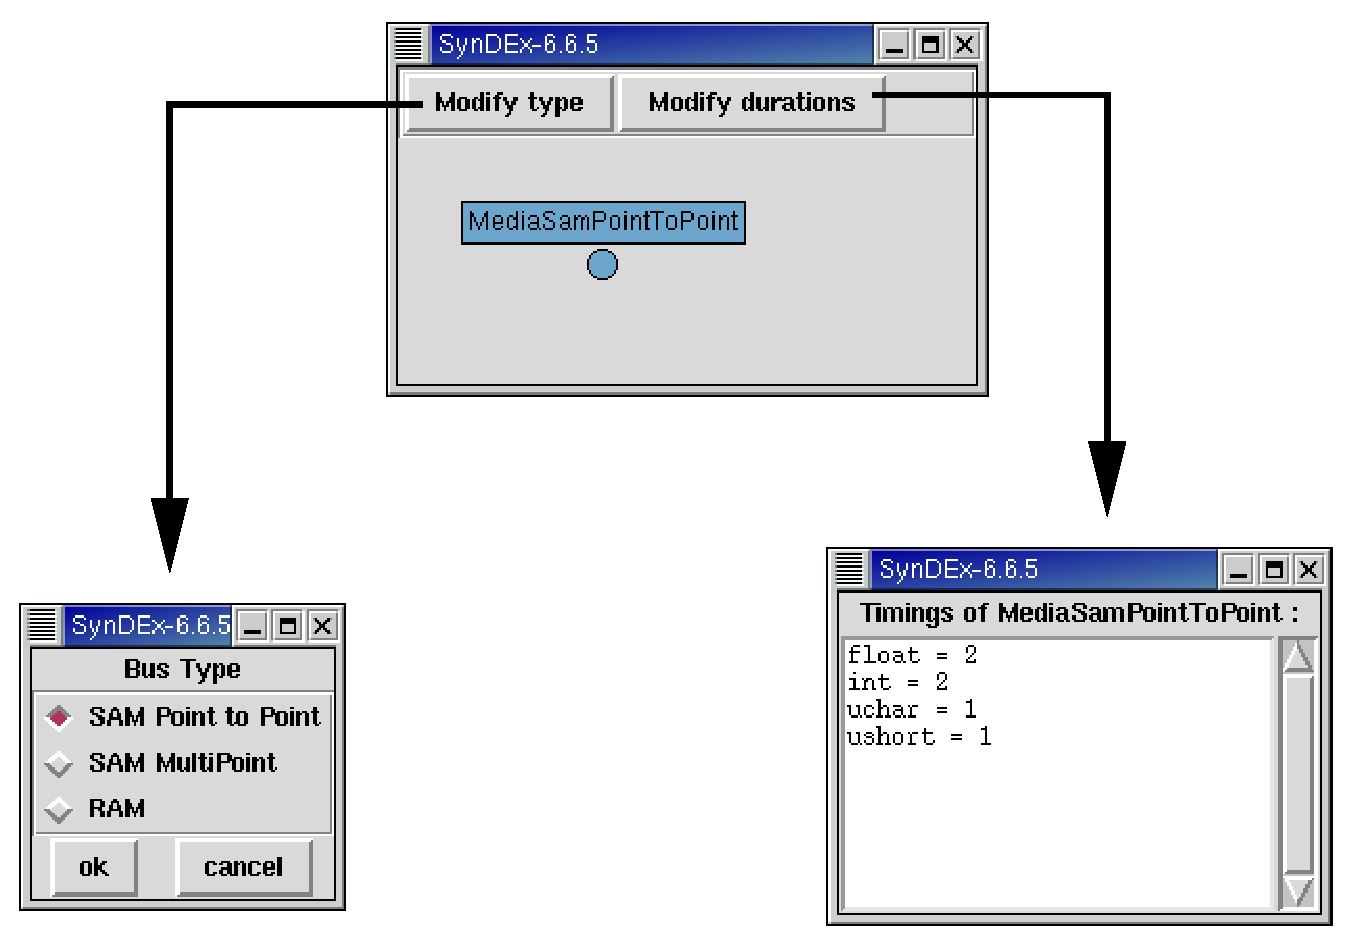
\includegraphics[width=\linewidth]{Media_of_communication_SPP.eps} 
  \end{center}
  
  \caption{Communication media SAM Point to Point} 
  \label{mediaSPP}
\end{figure}
\end{itemize}
\end{itemize}

\subsection{Creation of the main architecture definition}
\begin{itemize}
\item In the principal window, 

Menu: \textbf{Architecture / New Local Architecture} $\rightarrow$
DialogWindow ``ArchiSamPointToPoint'' $\rightarrow$ DefinitionWindow (figure
\ref{A_NLA}).

\item Define this architecture as main.

\item In the main architecture window, create two operators ``u1'', ``u2'', one of the type ``Uin'', the other of
the type ``Uout''.

\item In the main architecture window,

menu: \textbf{Edit / Create Media Reference} $\rightarrow$ DialogWindow: click
\textbf{local}, select \textbf{MediaSamPointToPoint} $\rightarrow$ DialogWindow:
``media\_sampp''

\item Define the operator ``u1'' as main (\textbf{Main Operator}).
\end{itemize}

\subsection{Creation of the connections between the operators and the media}
In the main architecture window, to create a connection between an operator and
a media, point the cursor on the port ``x'' of the ``u1'' operator, click the
middle button of the mouse (or CTRL+click the left button of the mouse) and
drag to the media of communication ``media\_sampp''. This draws an edge between
the operator and the media of communication. After creating the other
connection, we obtain the main architecture (figure \ref{archi1_2}).

\begin{figure}[ht]
  \begin{center} 
        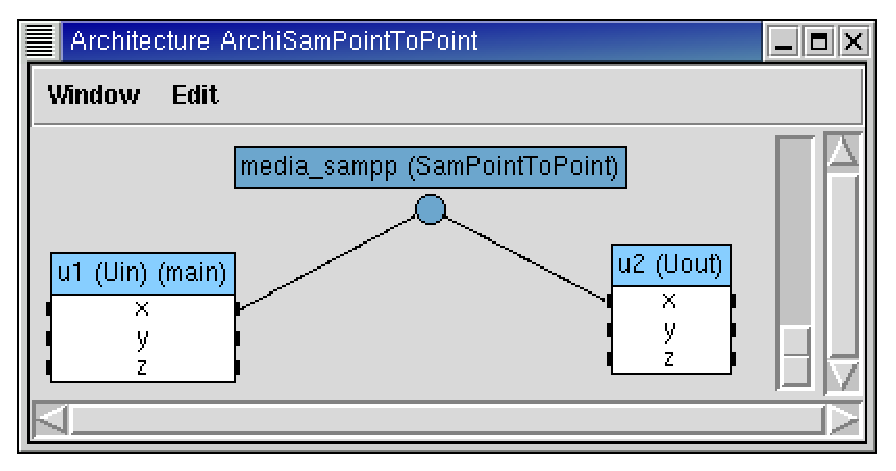
\includegraphics[width=0.527\linewidth]{architecture_ex1_2u_SPP.eps} 
  \end{center}
  \caption{Architecture with two operators and a media of type SAM Point to
Point} 
  \label{archi1_2}
\end{figure}

\section{Creation of architecture with three operators and a media of communication (SAM MultiPoint)} 
\label{archi1_3_SMP}

\begin{itemize}
\item In the principal window, 

Menu: \textbf{Architecture / New Local Architecture} $\rightarrow$
DialogWindow ``ArchiSamMultiPoint'' $\rightarrow$ DefinitionWindow (figure
\ref{A_NLA}).

\item Define this architecture as main.

\item Create two operators ``u1'' and ``u2'' of type ``Uin'' and an operator
``u3'' of type ``Uout'', like in the previous example.
\item Create a new media definition ``MediaSamMultiPoint'' of type ``SAM
MultiPoint'' and create a reference ``media\_sammp'' in the main algorithm
window.
\item Define the operator ``u1'' as main.
\item Connect the operators ports y to the media.
\end{itemize}

The architecture looks like the figure \ref{archi1_3}

\begin{figure}[ht]
  \begin{center} 
        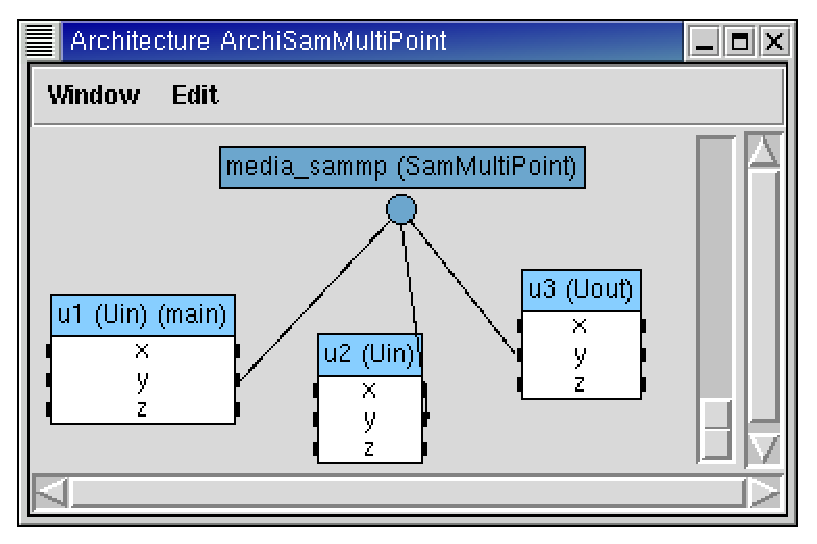
\includegraphics[width=0.56\linewidth]{architecture_ex1_3u_SMP.eps}
  \end{center} 
\caption{Architecture with three operators and a media of type SAM MultiPoint}
\label{archi1_3}
\end{figure}

\section{Creation of architecture with three operators and a media of
communication (RAM)}

\begin{itemize}
\item In the principal window, 

Menu: \textbf{Architecture / New Local Architecture} $\rightarrow$
DialogWindow ``ArchiRam'' $\rightarrow$ DefinitionWindow (figure
\ref{A_NLA}).

\item Define this architecture as main.

\item Create an operator ``u1''of type ``Uin'' and two operators ``u2'' and
``u3'' of type ``Uout''.
\item Create a new media definition ``MediaRam'' of type ``RAM'' and create a reference ``media\_ram'' in the main algorithm
window.
\item Define the operator ``u1'' as main.
\item Connect the operators ports z to the media.
\end{itemize}

The architecture looks like the figure \ref{archi1_4}.

\begin{figure}[htbp]
  \begin{center} 
        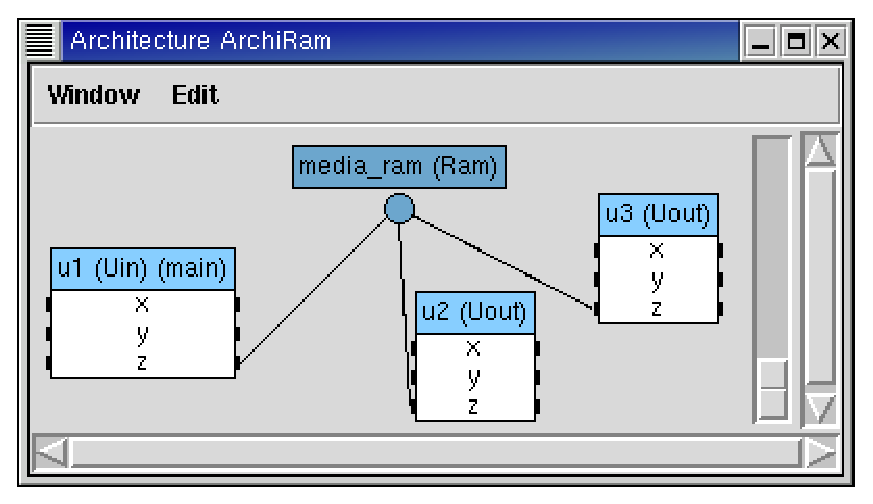
\includegraphics[width=0.6\linewidth]{architecture_ex1_3u_RAM.eps}
  \end{center} 
\caption{Architecture with three operators and a media of type RAM}
\label{archi1_4}
\end{figure}

\section{To perform the Adequation}
\subsection{The Adequation without constraint}
Select the architecture with three operators and a media of type Sam MultiPoint
(cf. \ref{archi1_3_SMP}) as main architecture (\textbf{Edit / Main Architecture}).

In the principal window, 

menu: \textbf{Adequation / No Flatten} (hierarchy is ignored) (or F3),

\hspace{81pt}\textbf{/ Flatten} (hierarchy is taken into account and all the
levels are flattened) (or F4).

This opens the schedule view window (figure \ref{adequation}) in which you can
see the schedule of the algorithm on the architecture and the schedule of the different
inter-operator communications on the media.
\begin{figure}[htbp]
  \begin{center} 
        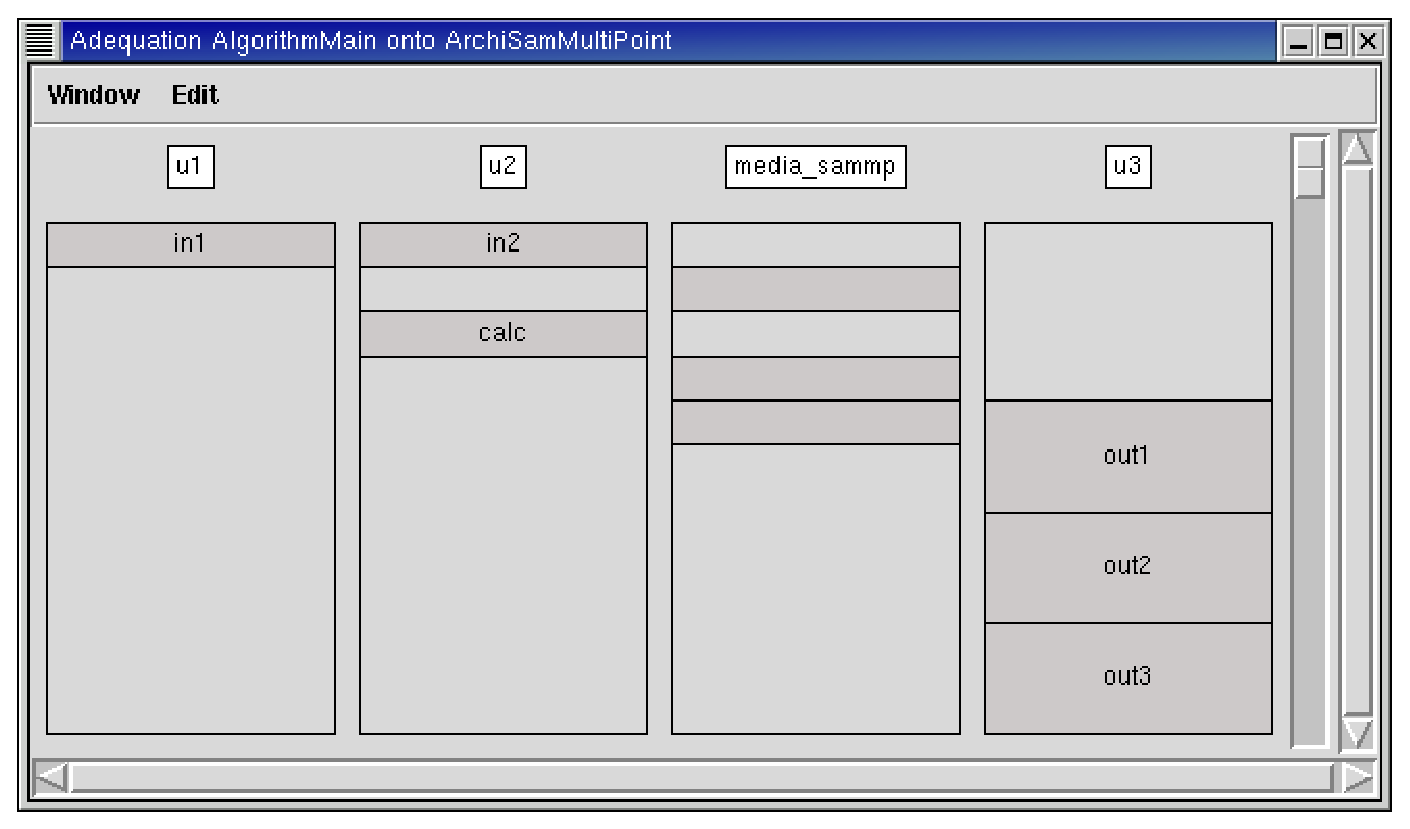
\includegraphics[width=1.03\linewidth]{Adequation.eps} 
  \end{center}
  \caption{Adequation} 
  \label{adequation}
\end{figure} 

\subsection{The Adequation with constraints}

\begin{itemize}
\item In the principal window, to create the constraints,

\begin{itemize}
\item Menu: \textbf{Algorithm / Create Software Component} $\rightarrow$
DialogWindow: ``xsc1 xsc2 xsc3'' (figure \ref{component})

\item Menu: \textbf{Constraints / Absolute Constraints} $\rightarrow$ DialogWindow:
select \textbf{ArchiSamMultiPoint}

This opens a dialog window in which you can create constraints on the different
operators of the architecture selected: 

\begin{itemize}
\item first click on ``xsc1'', then ``u1'', and the button \textbf{Create}
button, to constrain the Software Component ``xsc1'' on the operator ``u1''.
\item constrain the Software Component ``xsc2'' on the operator ``u2''.
\item constrain the Software Component ``xsc3'' on the operator ``u3''.
\item click on \textbf{OK} button.
\end{itemize}

\end{itemize}

\begin{figure}[htbp]
  \begin{center} 
        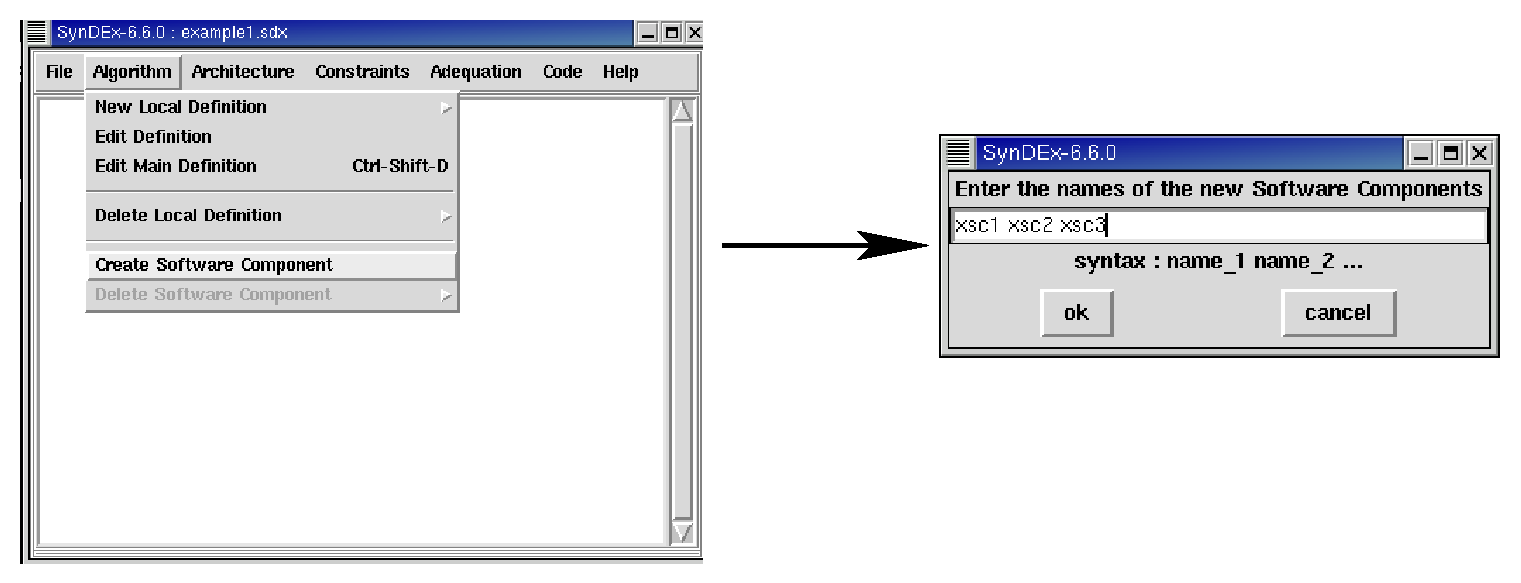
\includegraphics[width=1.1\linewidth]{create_software_component.eps} 
  \end{center}
  \caption{Create Software component} 
  \label{component}
\end{figure}

\begin{figure}[htbp]
  \begin{center} 
        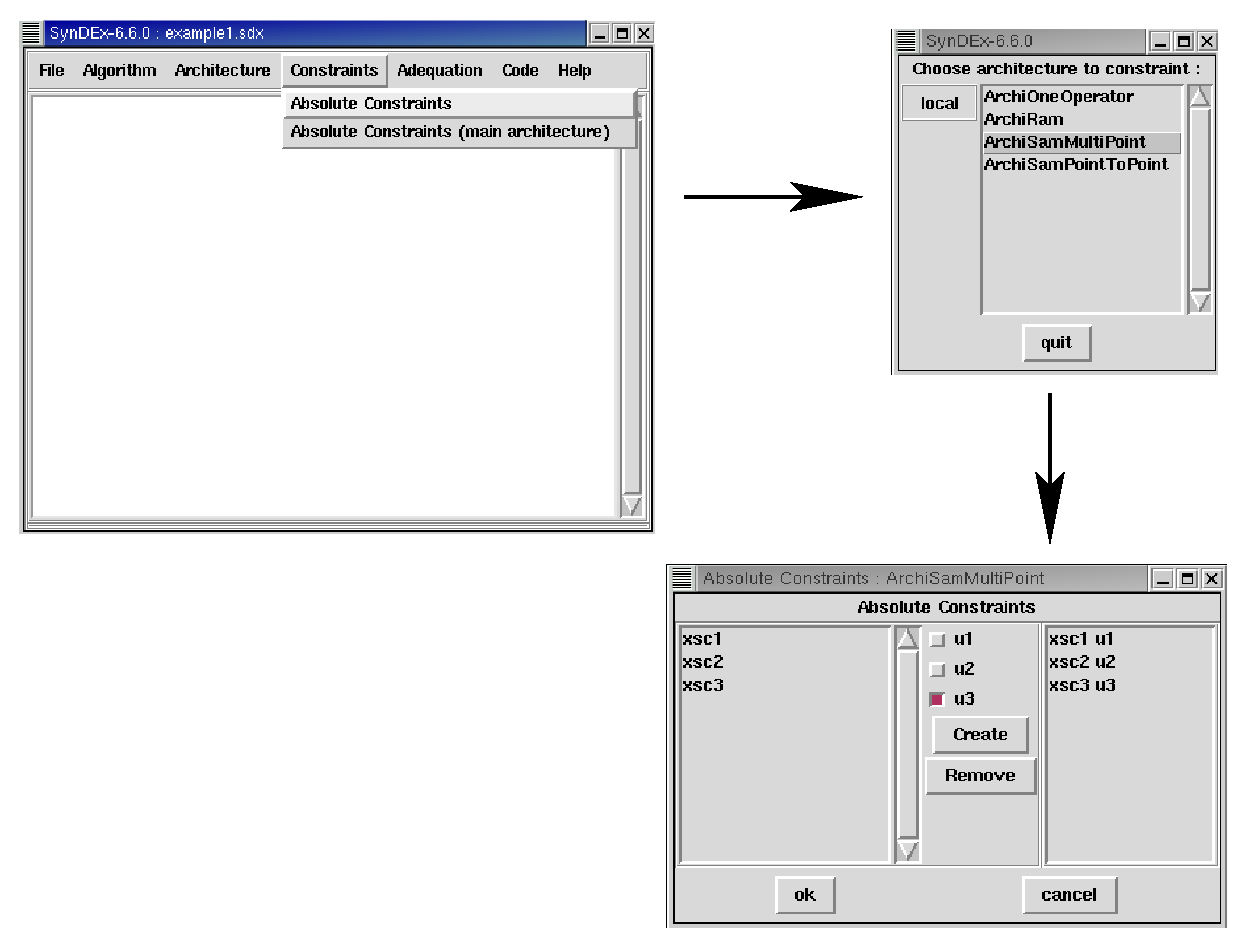
\includegraphics[width=\linewidth]{attach_software_component.eps} 
  \end{center}
  \caption{Attach Software component to the operators of the architecture selected} 
  \label{attach_component}
\end{figure}

\item In the main algorithm window,
\begin{itemize}
\item on the operation ``in1'', click right button of the mouse, then
\textbf{Attach Reference to the Software Component} (figure
\ref{attach_component}), and select \textbf{xsc1} ;

\item attach the operation ``in2'' to the Software Component ``xsc2'' ;
\item attach the operation ``out1'' to the Software Component ``xsc1'' ;
\item attach the operation ``out2'' to the Software Component ``xsc2'' ;
\item attach the operation ``out3'' to the Software Component ``xsc3'' ;
\item attach the operation ``calc'' to the Software Component ``xsc3''.
\end{itemize}

The algorithm with constraints looks like the figure \ref{algo_constraints}.

\begin{figure}[htbp]
  \begin{center} 
        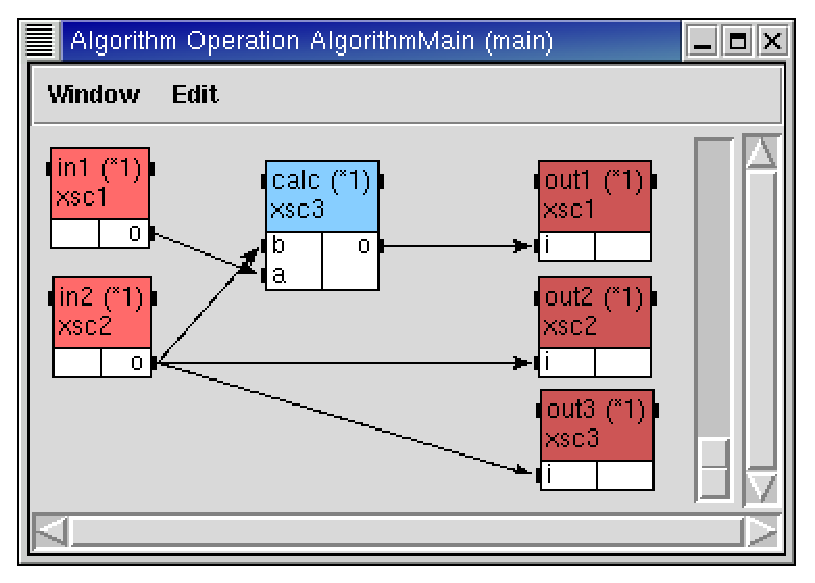
\includegraphics[width=0.5\linewidth]{Algorithm_constraints.eps} 
  \end{center}
  \caption{algorithm with constraints} 
  \label{algo_constraints}
\end{figure}

\item In the principal window to perform the adequation with constraints:

Menu: \textbf{Adequation / Flatten} $\rightarrow$ ScheduleViewWindow

The adequation looks like the figure \ref{adequation_constraints}.

\begin{figure}[h ]
  \begin{center} 
        \includegraphics[width=1.03\linewidth]{Adequation_constraints.eps} 
  \end{center}
  \caption{Adequation with constraints} 
  \label{adequation_constraints}
\end{figure}

\end{itemize}
\newpage
\chapter{Example 2 : hierarchy in algorithm}

\section{The algorithm}

\subsection{Creation of the definition ``A''}
\label{def_A}
\begin{itemize}
\item In the principal window,
\begin{itemize}
\item Menu: \textbf{Algorithm / New Local Definition / Function} $\rightarrow$
DialogWindow: ``A'' $\rightarrow$ DefinitionWindow
\item Menu: \textbf{Algorithm / New Local Definition / Constant} $\rightarrow$
DialogWindow: ``constante<X>''
\end{itemize}

\item In the ``A'' definition window,
\begin{itemize}
\item  create a reference ``cst<T>'' to the definition ``constante'',
\item create an input port ``a'', an output port ``o'' (Menu:
\textbf{Edit / Create Port}),
\item create a definition to the function ``calcul1'', then the reference to
this definition ``calc1'',

\item add a parameter name (figure \ref{parameter}): 

Menu: \textbf{Edit / Parameters Names} $\rightarrow$ DialogWindow: ``T''

\begin{figure}[htbp]
  \begin{center} 
        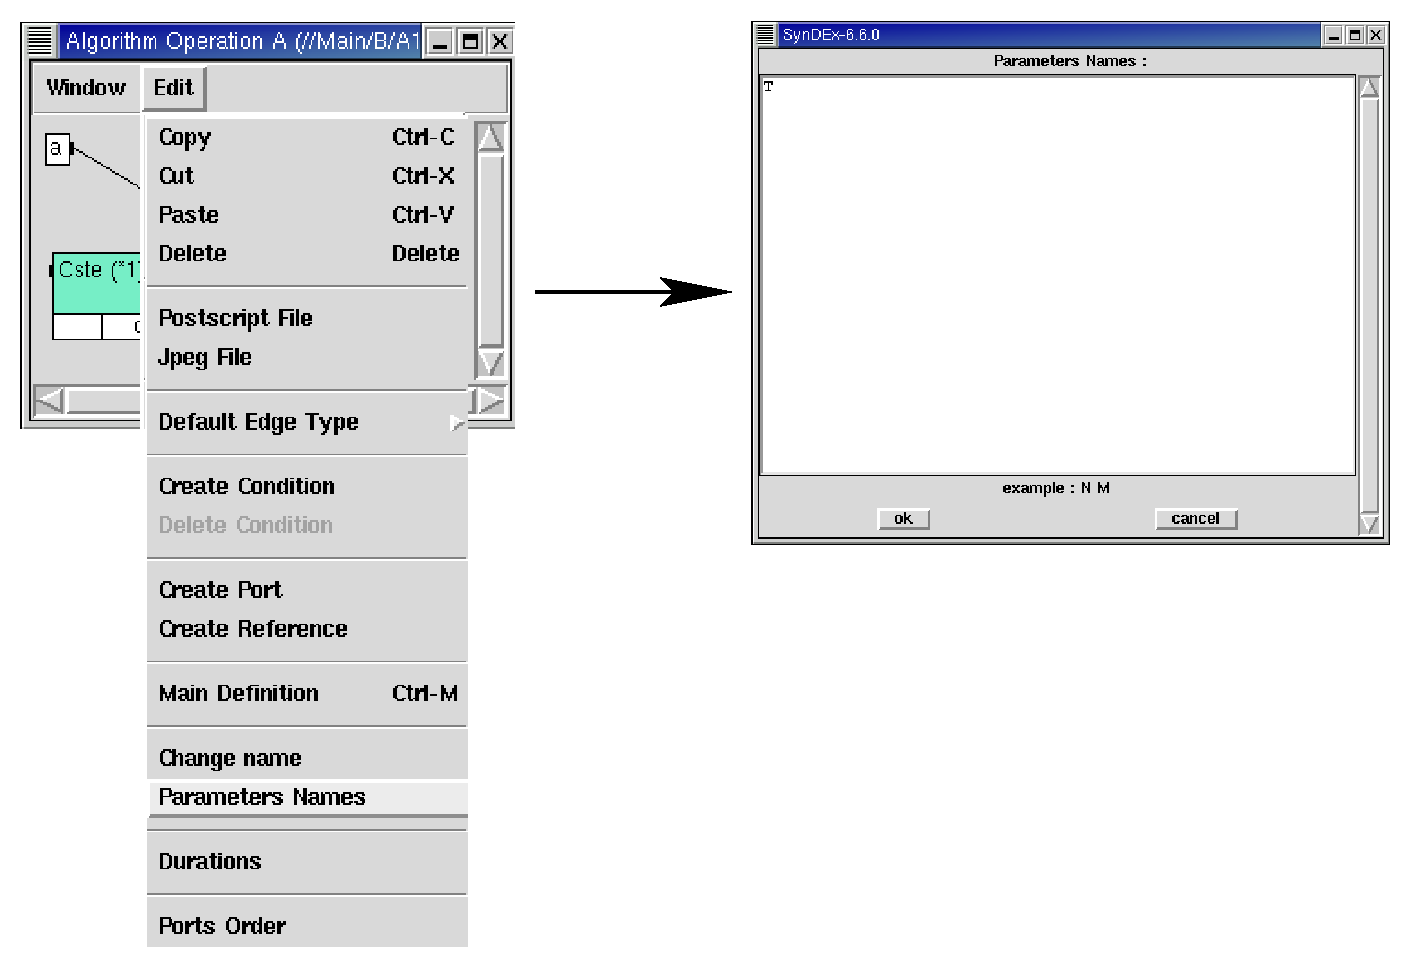
\includegraphics[width=\linewidth]{Edit_ParametersNames.eps} 
  \end{center}
  \caption{\textbf{Edit $\rightarrow$ parameters names}} 
  \label{parameter}
\end{figure}
\end{itemize}

\end{itemize}

The function ``A'' looks like the figure \ref{A}.

\begin{figure}[htbp]
  \begin{center} 
        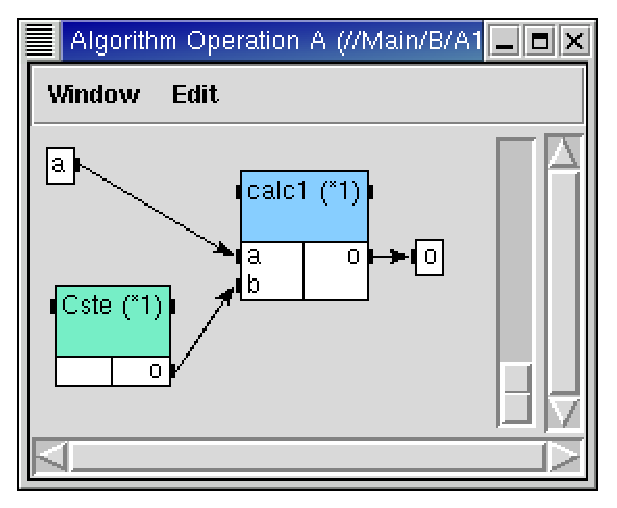
\includegraphics[width=0.5\linewidth]{OperationA.eps} 
  \end{center}
  \caption{Function ``A''} 
  \label{A}
\end{figure} 

\subsection{Creation of the definition ``B''}
\begin{itemize}
\item In the principal window,

 Menu: \textbf{Algorithm / New Local Definition / Function} $\rightarrow$
DialogWindow: ``B'' $\rightarrow$ DefinitionWindow

\item In the definition window,
\begin{itemize}
\item create the references ``A1'' and ``A2'' (definition ``A'') (Menu:
\textbf{Edit / Create Reference} $\rightarrow$ DialogWindow: click
\textbf{Local}, select \textbf{A}) $\rightarrow$ DialogWindow: ``A1<X> A2<Y>''

\item create two input ports ``a'' and ``b'', one output port ``o'' and the
function ``calc1'' of the definition ``calcul1''.

\item add the parameters names ``X'' and ``Y'' (menu: \textbf{Edit / Parameters
Names}).
\end{itemize}

The function ``B'' looks like the figure \ref{B}.
\begin{figure}[htbp]
  \begin{center} 
        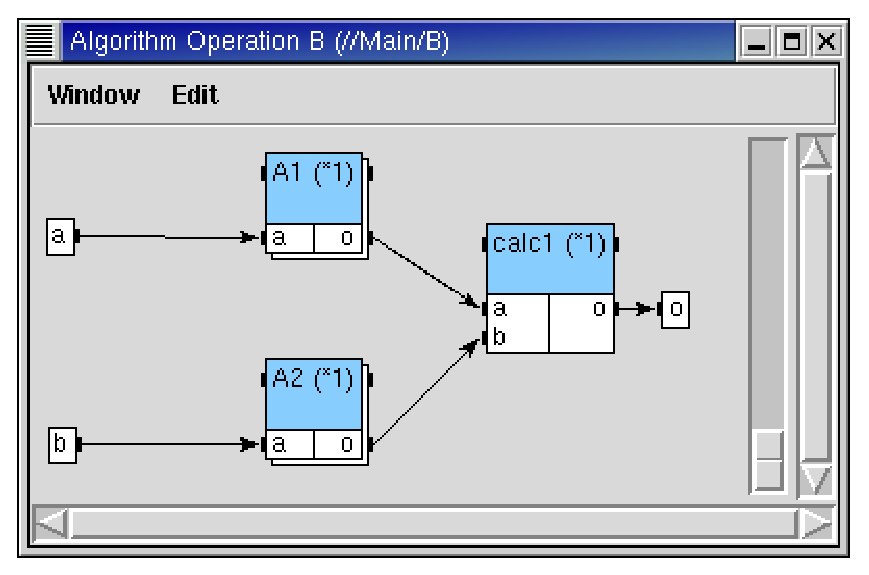
\includegraphics[width=0.67\linewidth]{OperationB.eps} 
  \end{center}
  \caption{Function ``B''} 
  \label{B}
\end{figure}

\end{itemize}

\subsection{Creation of the main algorithm definition}
\begin{itemize}
\item In the principal window,

Menu: \textbf{Algorithm / New Local Definition / Function} $\rightarrow$
DialogWindow: ``Main''

\item In the definition window, define this algorithm as main algorithm (CTRL + M).

\item Add the functions ``i1'', ``i2'', ``o'' and ``B'' in the algorithm window

\item In the principal window, create two \textbf{sensors}, ``i1'' and
``i2''. Create an \textbf{actuator} ``o''.

Menu: \textbf{Algorithm / New Local Definition}

\item In the main algorithm window, 

Menu: \textbf{Edit / Create Reference} $\rightarrow$ button: \textbf{local},
select \textbf{B} $\rightarrow$ DialogWindow: ``B<1;2>''

\hspace{197pt} select \textbf{input} $\rightarrow$ DialogWindow: ``i1 i2''

\hspace{197pt} select \textbf{output} $\rightarrow$ DialogWindow: ``out'

\item Create dependences between the references.

\end{itemize}

The algorithm looks like the figure \ref{algo2}.
\begin{figure}[htbp]
  \begin{center} 
        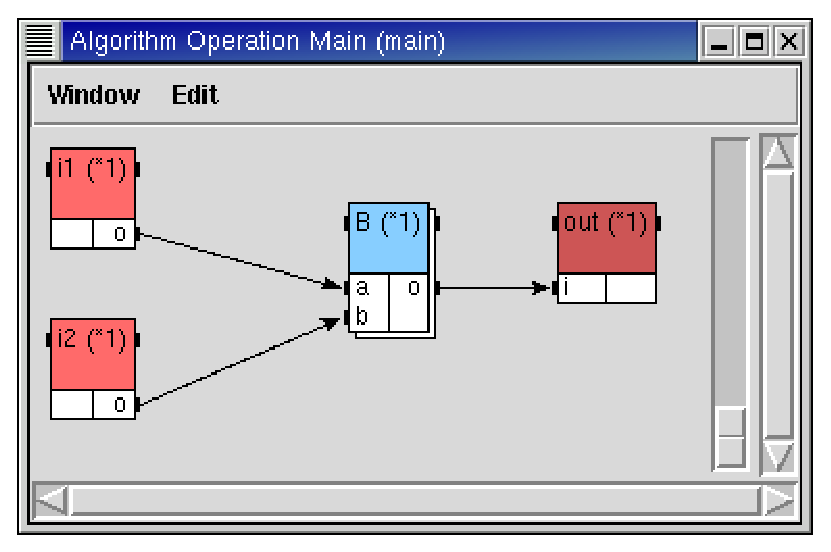
\includegraphics[width=0.5\linewidth]{algorithm_ex2.eps} 
  \end{center}
  \caption{algorithm of the example 2} 
  \label{algo2}
\end{figure} 

\chapter{Example 3 : delay and constant in algorithm}
\section{The algorithm}
\subsection{Creation of the functions ``in1'', ``out1'', ``calc''}

Create a \textbf{sensor} ``input'', an \textbf{actuator} ``output'', and the
\textbf{function} ``calc'', like in the
examples 1 and 2. (cf. \ref{algo_ex1}, \ref{def_A})

\subsection{Creation of the delay definition}
\begin{itemize}
\item In the principal window, 

menu: \textbf{Algorithm / New Local Definition / Delay} $\rightarrow$
DialogWindow: ``calcPrec<X>'' $\rightarrow$ DefinitionWindow. The parameter X
will be use to specify the initial value. 

\item In the definition window,

create one \textbf{input} port and one \textbf{output} port. Enter: \textbf{?
  int x !  int x}. Notice input and outport name are the same.


\end{itemize}

\subsection{Creation of the algorithm}
Create a reference ``in1'' on the definition ``input'', a reference ``calc'' on
the definition ``calc'', a reference ``out1'' on the definition ``output'' and
a reference ``calcPrec<0>'' on the definition ``calcPrec''(Menu: \textbf{Edit /
Create Reference}). Create dependences between the references.

The algorithm looks like the figure \ref{algo3}.

\begin{figure}[htbp]
  \begin{center} 
        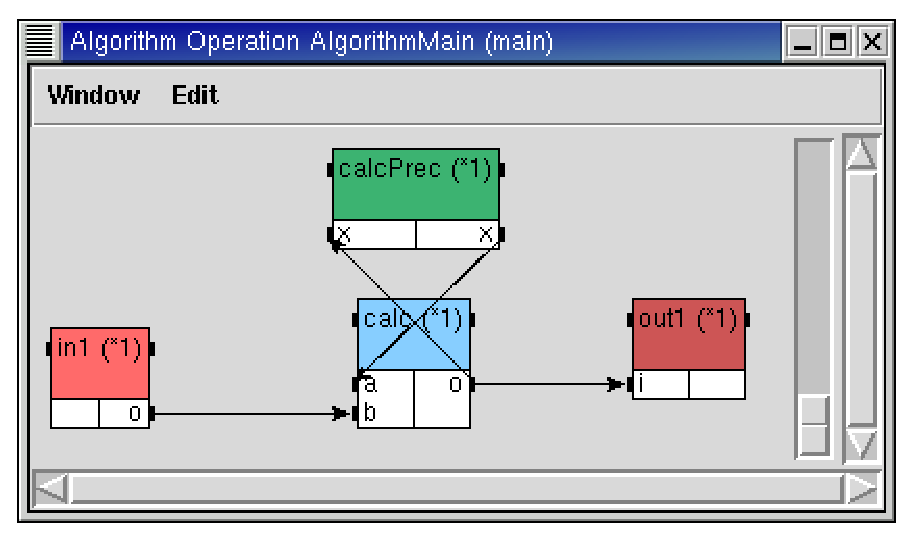
\includegraphics[width=0.57\linewidth]{algorithm_ex3.eps} 
  \end{center}
  \caption{algorithm of the example 3}
  \label{algo3}
\end{figure}
\chapter{Example 4 : repetition and library in algorithm}
\section{Creation of the algorithm without library}
\subsection{Creation of the sensor ``ins'' and function ``mul'' (function on scalars):}

In the principal window,

Menu: \textbf{Algorithm / New Local Definition / sensor} (for ``ins'' of type
``input''),

\hspace{175pt}\textbf{/ function} (for ``mul'' of type ``mul'').

\subsection{Creation of the sensor ``inv'' and actuator ``outv'' (operations on
vectors):}
\begin{itemize}
\item To create the definition ``inv'',
\begin{itemize}
\item In the principal window,

Menu: \textbf{Algorithm / New Local Definition / sensor} $\rightarrow$
DialogWindow: ``inv'' $\rightarrow$ DefinitionWindow

\item In the definition window,

create a parameter name ``N''. menu: \textbf{Edit / Parameters Names}

create an output port ``o''. menu: \textbf{Edit / Create Port} $\rightarrow$
DialogWindow: ``! int[N] o''
\end{itemize}

\item To create the definition ``outv'',
\begin{itemize}
\item In the principal window,

Menu: \textbf{Algorithm / New Local Definition / actuator} $\rightarrow$
DialogWindow: ``outv'' $\rightarrow$ DefinitionWindow

\item In the definition window,

create a parameter name ``N''. Menu: \textbf{Edit / Parameters Names}

create one output port ``i''. Menu: \textbf{Edit / Create Port} $\rightarrow$
DialogWindow: ``? int[N] i''
\end{itemize}

\item To create the definition ``AlgorithmMain1'',
\begin{itemize}
\item In the principal window,

Menu: \textbf{Algorithm / New Local Definition / function} $\rightarrow$
DialogWindow: ``AlgorithmMain1'' $\rightarrow$ DefinitionWindow

\item In the definition window, define ``AlgorithmMain1'' as main algorithm,
  and create the parameter name ``N'' with the value 3 (figure
\ref{ParameterAndValue}). menu: \textbf{Edit / Parameters Names and Values}
$\rightarrow$ DialogWindow: ``N=3''
\end{itemize}

\begin{figure}[htbp]
  \begin{center} 
        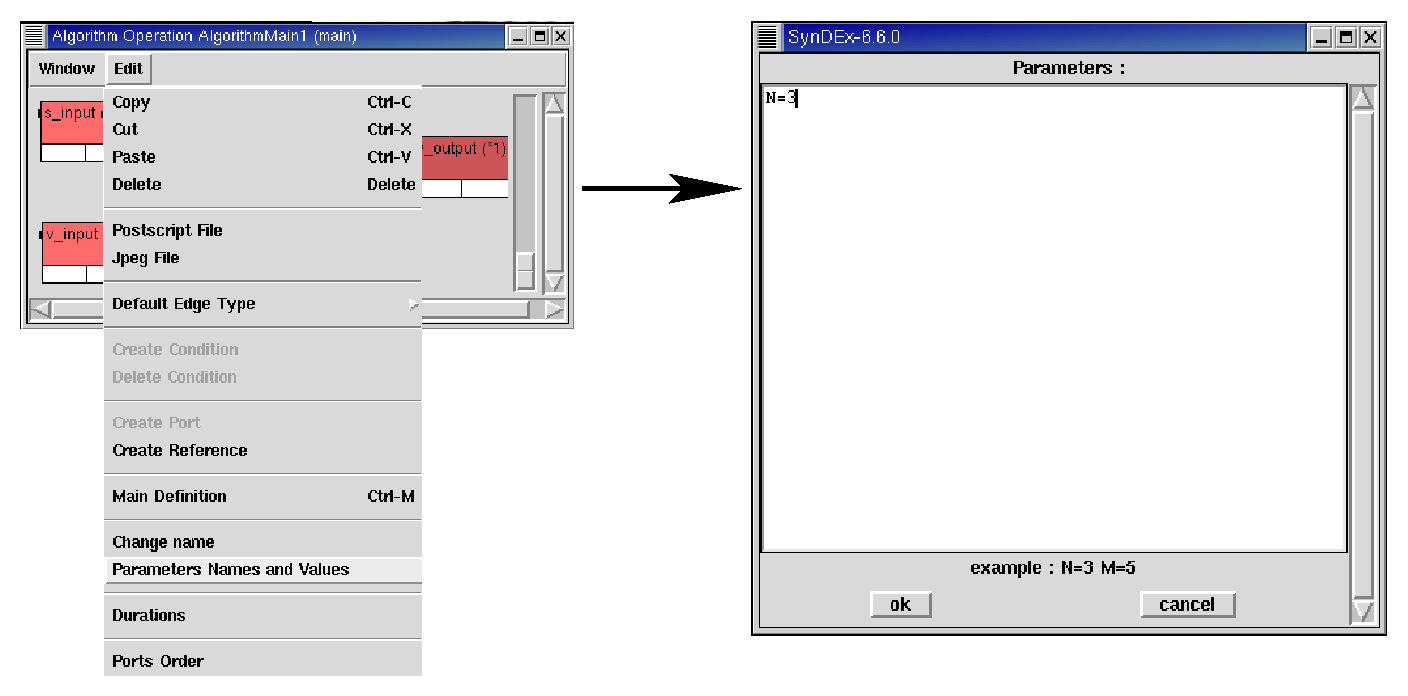
\includegraphics[width=\linewidth]{Edit_ParametersNamesAndValues.eps} 
  \end{center}
  \caption{Parameters Names and Values}
  \label{ParameterAndValue}
\end{figure}

\item In the main algorithm, create a reference ``s\_input'' on the definition
``ins'', a reference ``mul'' on the definition ``mul'', a reference
``v\_input<N>'' on the defintion ``inv'', a reference ``v\_output<N>'' on the
definition ``outv''.

\end{itemize}

Create dependences between the references. The algorithm looks like the figure \ref{algomain1_4}.

\section{Creation of the algorithm with library ``int''}
\subsection{Creation of the operations with the library ``int'':}
\begin{itemize}
\item in the principal window, 

Menu: \textbf{File / Include Library / int} (figure \ref{library}).

\begin{figure}[htbp]
  \begin{center} 
        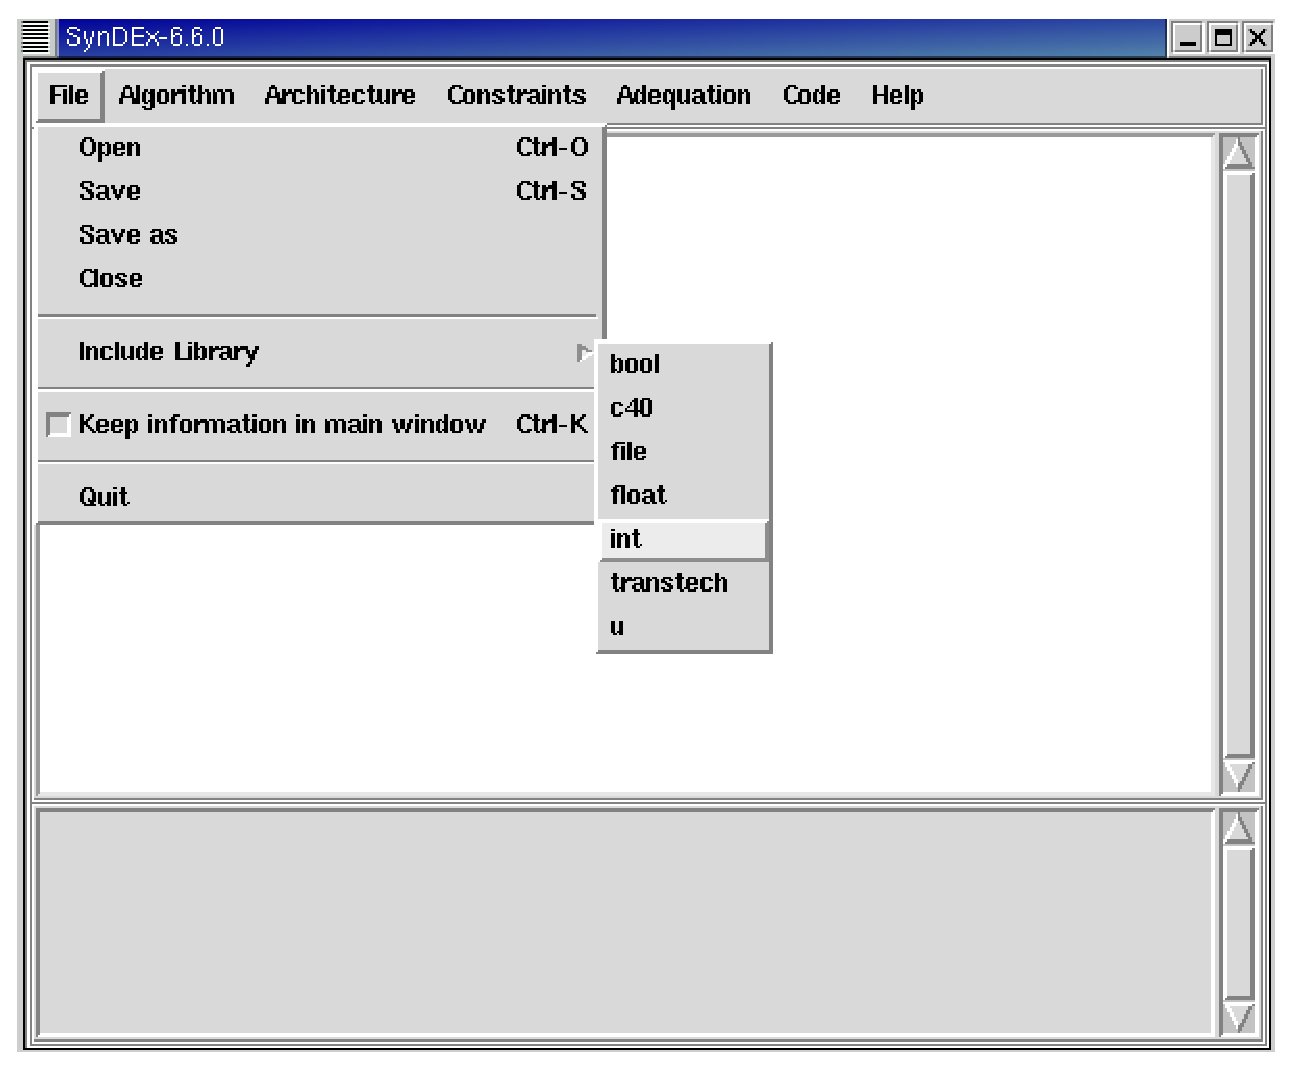
\includegraphics[width=0.6\linewidth]{File_IncludeLibrary_int.eps} 
  \end{center}
  \caption{\textbf{File $\rightarrow$ Include Library $\rightarrow$ int}}
  \label{library}
\end{figure}
\item in the main algorithm window,

Menu: \textbf{Edit / Create Reference} $\rightarrow$ DialogWindow: select
\textbf{int} (figure \ref{library2}) then :

\begin{itemize}
\item select \textbf{input} $\rightarrow$ DialogWindow: ``s\_input<1>'' ;
\item select \textbf{Arit\_mul} $\rightarrow$ DialogWindow: ``mul<1>'' ;
\item select \textbf{input} $\rightarrow$ DialogWindow: ``v\_input<N>'' ; 
\item select \textbf{output} $\rightarrow$ DialogWindow: ``v\_output<N>''.
\end{itemize}

\begin{figure}[htbp]
  \begin{center} 
        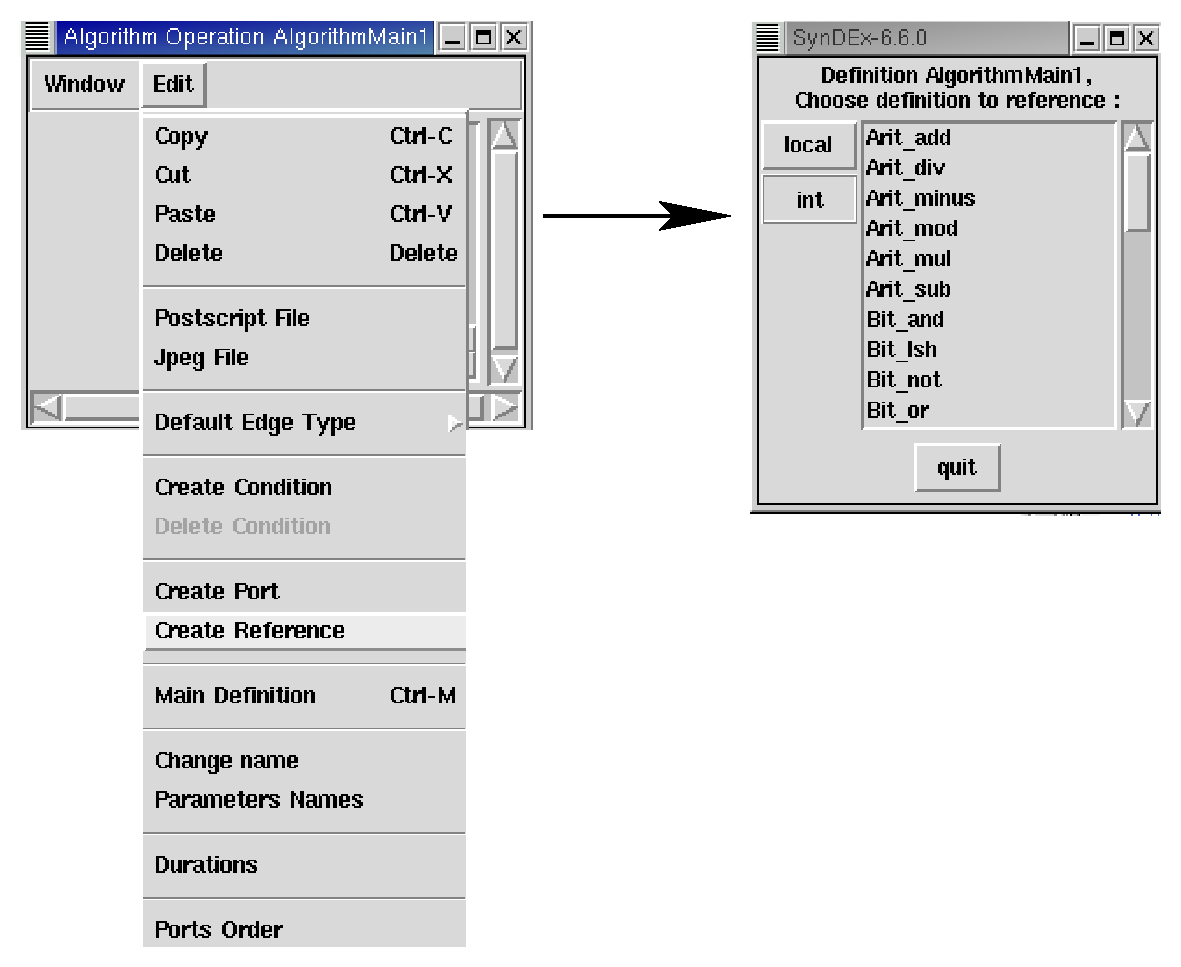
\includegraphics[width=0.9\linewidth]{Library_int.eps} 
  \end{center}
  \caption{\textbf{Create Reference $\rightarrow$ int button}}
  \label{library2}
\end{figure}

\end{itemize}

Create dependences between the references in order to obtain the main algorithm
like the figure \ref{algomain1_4}.

\begin{figure}[htbp]
  \begin{center} 
        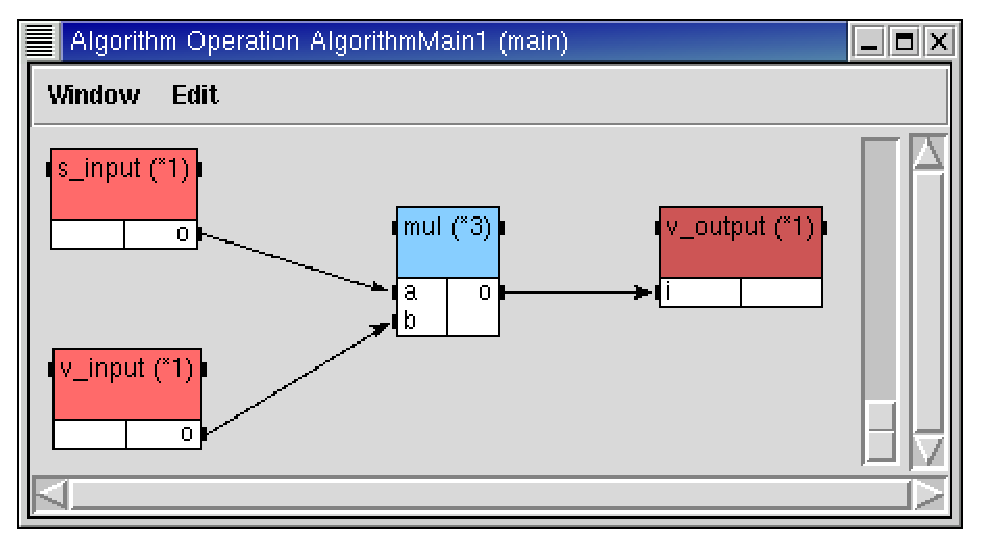
\includegraphics[width=0.48\linewidth]{algorithm_ex4.eps} 
  \end{center}
  \caption{algorithmMain1 of the example 4}
  \label{algomain1_4}
\end{figure}

\section{Creation of the algorithm with library float}

\begin{itemize}
\item Include the library ``float'' (Menu: \textbf{File / Include Library / Float}).

\item Create the definition of the function \textbf{dpacc} (figure
\ref{dpacc}), with the functions ``mul'' (definition Arit\_mul) and ``add''
(definition Arit\_add) which are in the library
``float'' (Menu: \textbf{Edit / Create Reference} $\rightarrow$ DialogWindow:
select \textbf{Float}), and three input ports ``?  float s1 ?  float s2 ?
float acc'', and an output port ``!  float acc'' (Menu: \textbf{Edit / Create
  Port}). Then:
\begin{itemize}
\item create a dependence between the input port ``s1'' and the port ``a'' of ``mul'' ;

\item create a dependence between the input port ``s2'' and the port ``b'' of ``mul'' ;

\item create a dependence between the input port ``acc'' and the port ``b'' of ``add''; 

\item create a dependence between the port ``o'' of ``mul'' and the port ``a'' of
``add'' ;

\item create a dependence between the output port ``acc'' and the port ``o'' of
``add''.
\end{itemize}
\begin{figure}[htbp]
  \begin{center} 
        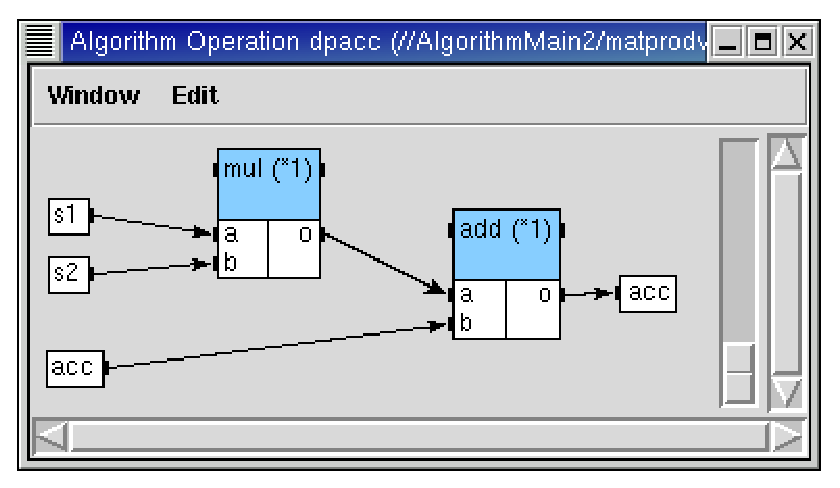
\includegraphics[width=0.55\linewidth]{algorithm_ex4_dpacc.eps} 
  \end{center}
  \caption{algorithm of the function ``dpacc''}
  \label{dpacc}
\end{figure}

\item Create the definition of the function \textbf{dp} (figure \ref{dp}),
with a parameter name \textbf{dpaccn} (menu: \textbf{Edit / Parameters Names}),
and with a constant ``zero<{0}>'' which is in the library \textbf{float}, the
function ``dpacc'' of the definition \textbf{dpacc}, and two \textbf{input
ports} ``?  float[dpaccn] v1 ? float[dpaccn] v2'', and an \textbf{output} port
``!  float dp''. Then:
\begin{itemize}
\item create a dependence between the input port ``v1'' and the port ``s1'' of
``dpacc'' ;

\item create a dependence between the input port ``v2'' and the port ``s2'' of
``dpacc'' ;

\item create a dependence between the port ``o'' of ``zero'' and the input port
``acc'' of ``dpacc'' ;

\item create a dependence between the output port ``dp'' and the output port ``acc''
of ``dpacc''.
\end{itemize}
\begin{figure}[htbp]
  \begin{center} 
        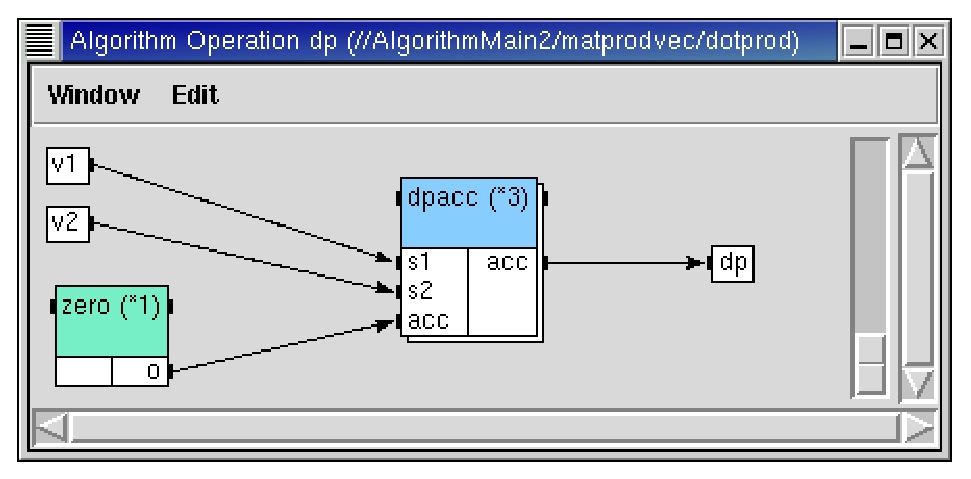
\includegraphics[width=0.55\linewidth]{algorithm_ex4_dp.eps} 
  \end{center}
  \caption{algorithm of the function ``dp''}
  \label{dp}
\end{figure}

\item Create the definition of the function \textbf{prodmatvec} (figure
\ref{prodmatvec}), with the parameters names ``a'' and ``b'', and
with the function ``dotprod<b>'' of the definition \textbf{dp}, two
\textbf{input} ports ``?  float[a*b] outm ?  float[a] inv'', and an
\textbf{output} port ``!  float[b] inm''. Then:
\begin{itemize}
\item create a dependence between the input port ``outm'' and the port ``v1'' of
``dotprod'' ;

\item create a dependence between the input port ``inv'' and the port ``v2'' of
``dotprod'' ;

\item create a dependence between the output port ``inm'' and the output port ``dp''
of ``dotprod''.
\end{itemize}
\begin{figure}[htbp]
  \begin{center} 
        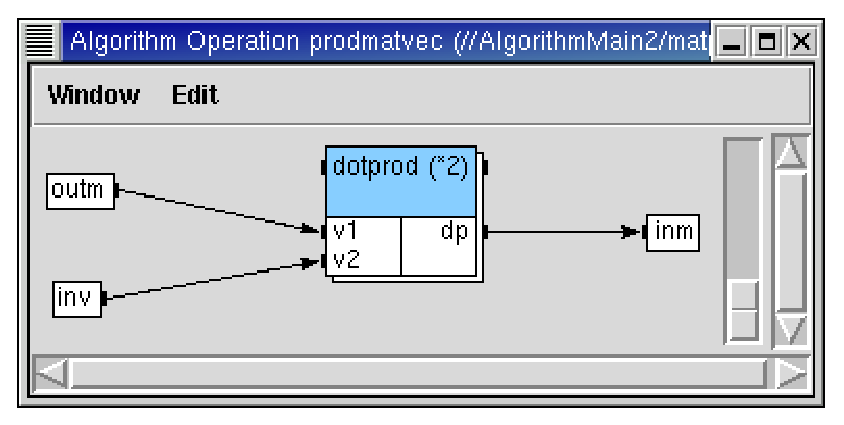
\includegraphics[width=0.55\linewidth]{algorithm_ex4_prodmatvec.eps} 
  \end{center}
  \caption{algorithm of the function ``prodmatvec''}
  \label{prodmatvec}
\end{figure}

\item Create the definition of the sensor \textbf{inm}, with two parameters
names ``N'' and ``M'', and with an \textbf{output} port ``!  float
[N*M] o''.

\item Define the ``AlgorithmMain2'' as main algorithm. Then:
\begin{itemize}
\item define two parameters names: N=3 and M=4 ;

\item create the references ``m1<N;M>'' on the definition \textbf{inm},
``inv<N>'' on the definition \textbf{input} in the library \textbf{float},
``matprodvec<N;M>'' on the definition \textbf{prodmatvec}, ``outv<M>'' on
the definition \textbf{output} in the library \textbf{float} ;

\item create a dependence between ``m1'' and the port ``outm'' of ``matprodvec'' ;

\item create a dependence between ``v'' and the port ``inv'' of ``matprodvec'' ;

\item create a dependence between ``outv'' and the output port ``inm'' of
``matprodvec''.
\end{itemize}
The ``AlgorithmMain2'' looks like the figure \ref{algomain2_4}.

\begin{figure}[htbp]
  \begin{center} 
        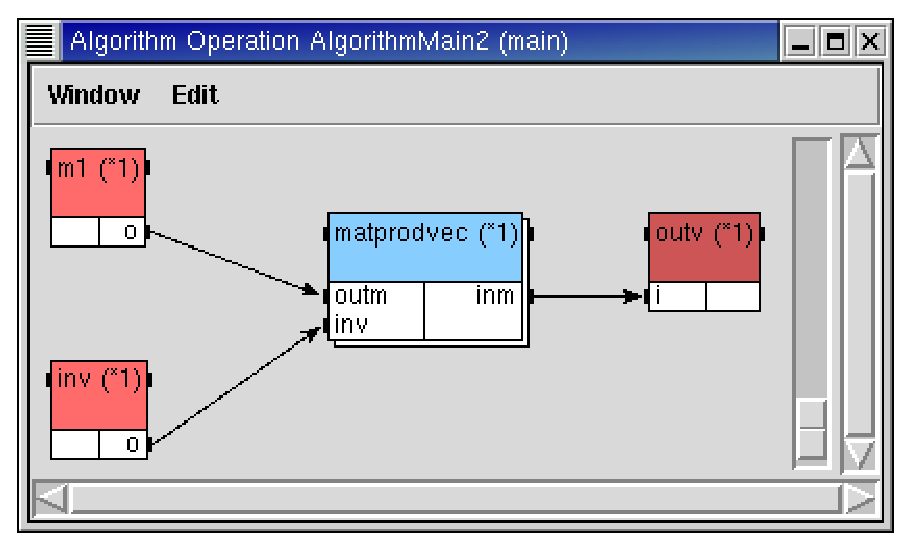
\includegraphics[width=0.55\linewidth]{algorithmMain2_ex4.eps} 
  \end{center}
  \caption{``AlgorithmMain2'' of the example 4}
  \label{algomain2_4}
\end{figure}

\end{itemize}

\chapter{Example 5 : condition and nested condition in
algorithm}
\section{Creation of  the first algorithm}
\subsection{Creation of the sensors ``x'' and ``i'' (type ``input''),
the actuator ``o'' (type ``output'')}

Menu: \textbf{Algorithm / New Local Definition / sensor} (for ``x'' and ``i''),

\hspace{157pt}\textbf{ / actuator} (for ``o'').

\subsection{Creation of the definition ``switch1''}
\begin{itemize}
\item In the principal window,

Menu: \textbf{Algorithm / New Local Definition / function} $\rightarrow$
DialogWindow: ``switch1'' $\rightarrow$ DefinitionWindow

\item In the definition window, 
\begin{itemize}
\item Menu: \textbf{Edit / Create Port} $\rightarrow$ DialogWindow: ``? int x ?
int i !  int o''

\item Menu: \textbf{Edit / Create Condition} $\rightarrow$ DialogWindow: ``x=1
x=2 x=3 x=4'' (figure \ref{condition}).

\begin{figure}[htbp]
  \begin{center} 
        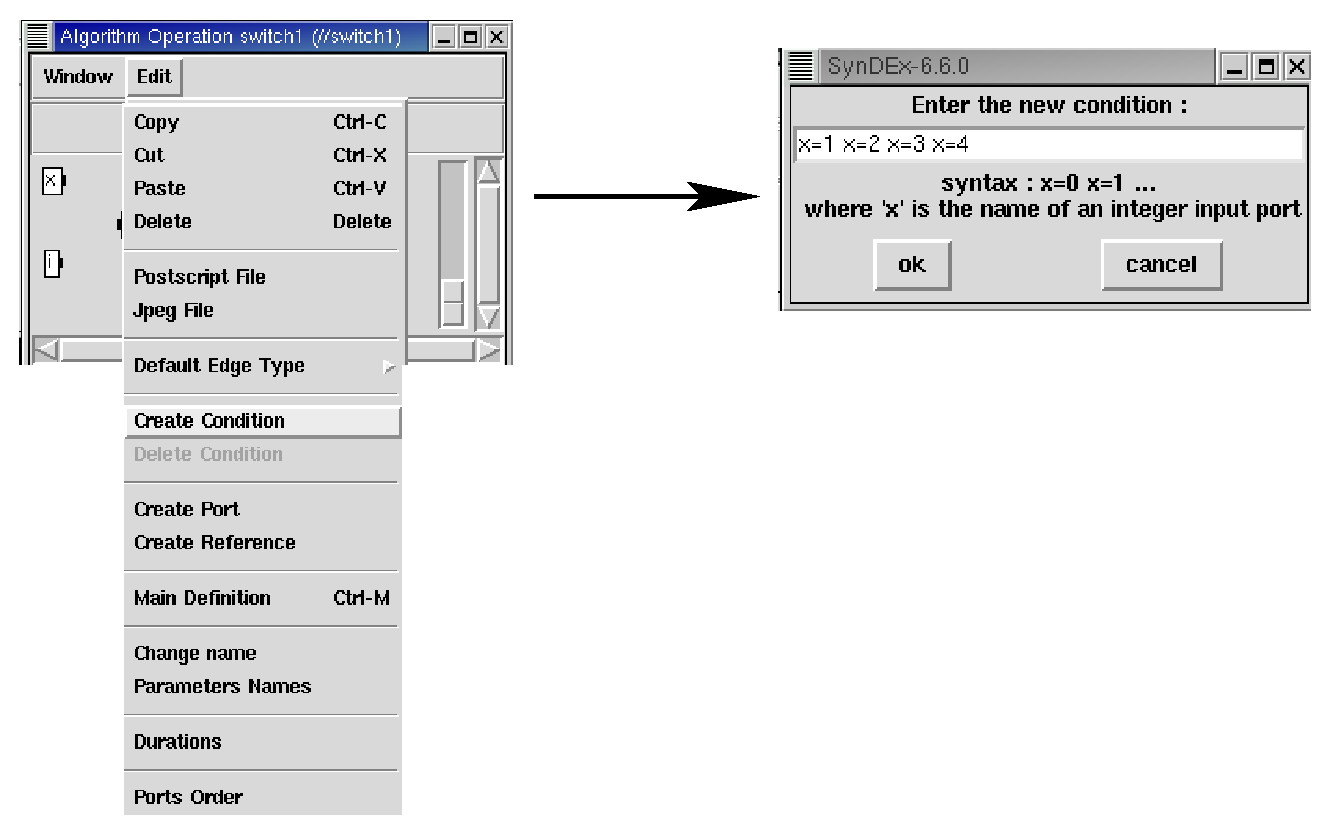
\includegraphics[width=1.1\linewidth]{Edit_CreateCondition.eps} 
  \end{center}
  \caption{\textbf{Edit $\rightarrow$ Create Condition}}
  \label{condition}
\end{figure}
\begin{itemize}
\item click on the condition ``x=1'' (figure \ref{condition1}) 

and create the reference ``div1<1>'' (definition \textbf{Arit\_div} from
``int'' library) ;

\begin{figure}[htbp]
  \begin{center} 
        \includegraphics[width=0.5\linewidth]{Condition1.eps} 
  \end{center}
  \caption{Condition x=1}
  \label{condition1}
\end{figure}

\item click on the condition ``x=2'' (figure \ref{condition2})

and create the reference ``div2<1>'' (definition \textbf{Arit\_div} from
``int'' library) ;

\begin{figure}[htbp]
  \begin{center} 
        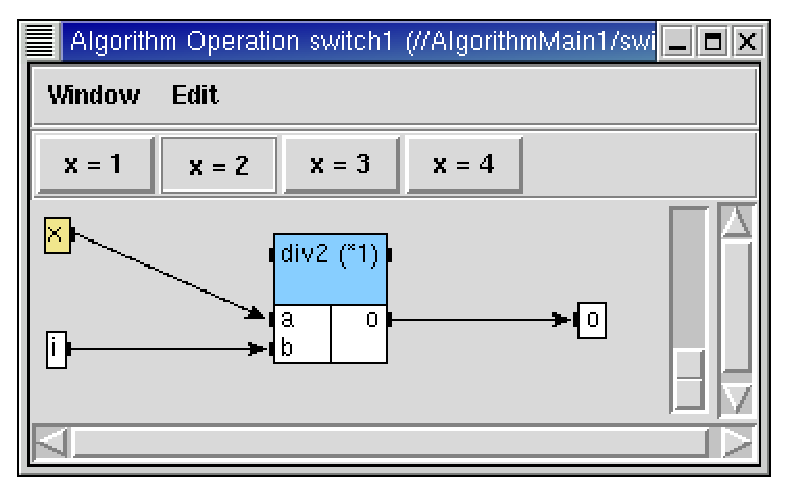
\includegraphics[width=0.5\linewidth]{Condition2.eps} 
  \end{center}
  \caption{Condition x=2}
  \label{condition2}
\end{figure}

\item click on the condition ``x=3'' (figure \ref{condition3}) 

and connect the port ``i'' to the port ``o'' ;

\begin{figure}[htbp]
  \begin{center} 
        \includegraphics[width=0.5\linewidth]{Condition3.eps} 
  \end{center}
  \caption{Condition x=3}
  \label{condition3}
\end{figure}

\item click on the condition ``x=4'' (figure \ref{condition4}) 

and create the reference ``mul4<1>'' (definition \textbf{Arit\_mul} from ``int'' library).

\begin{figure}[htbp]
  \begin{center} 
        \includegraphics[width=0.5\linewidth]{Condition4.eps} 
  \end{center}
  \caption{Condition x=4}
  \label{condition4}
\end{figure}

\end{itemize}

\item create dependences between the references.
\end{itemize}
\end{itemize}
The algorithm looks like the figure \ref{algo5}.

\begin{figure}[htbp]
  \begin{center} 
        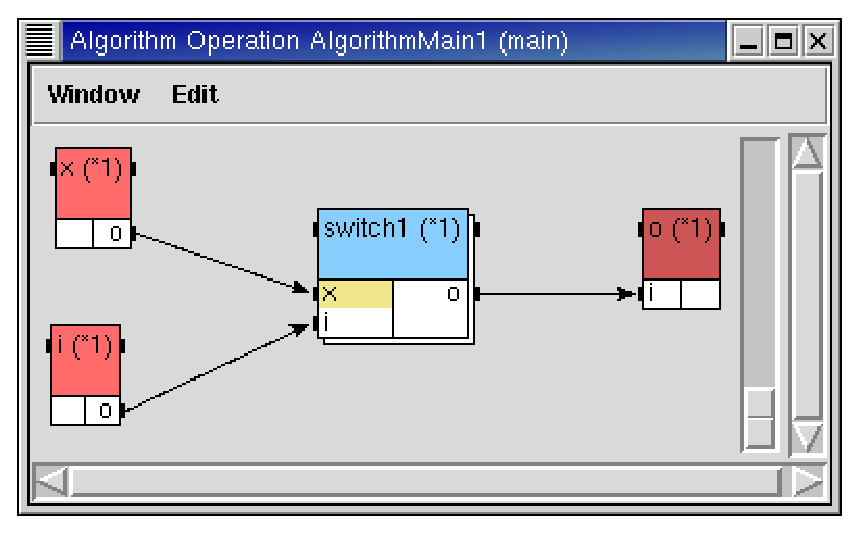
\includegraphics[width=0.5\linewidth]{algorithm_ex5.eps} 
  \end{center}
  \caption{algorithm of the example 5}
  \label{algo5}
\end{figure}

\section{Creation of the second algorithm}
\subsection{Creation of the sensors ``x'' and ``i'' of the type ``input'',
the actuator ``o'' of the type ``output''}
In the principal window,

Menu: \textbf{Algorithm / New Local Definition / sensor} (for ``x'' and ``i''),

\hspace{172pt} \textbf{/ actuator} (for ``o'').

\subsection{Creation of the definition ``switch2''}
\begin{itemize}
\item In the principal window,

Menu: \textbf{Algorithm / New Local Definition / function} $\rightarrow$
DialogWindow: ``switch2'' $\rightarrow$ DefinitionWindow

\item In the definition window, 
\begin{itemize}
\item Menu: \textbf{Edit / Create Port} $\rightarrow$ DialogWindow: ``? int x ?
  int y !  int o'' ;

\item Menu: \textbf{Edit / Create Condition} $\rightarrow$ DialogWindow: ``y=1
y=2'' ;

\item click on the condition ``y=1'' (figure \ref{condition1_algo2}) 

and create the function ``mul1'' of the definition \textbf{Arit\_mul} from
``int'' library ;

\begin{figure}[htbp]
  \begin{center} 
        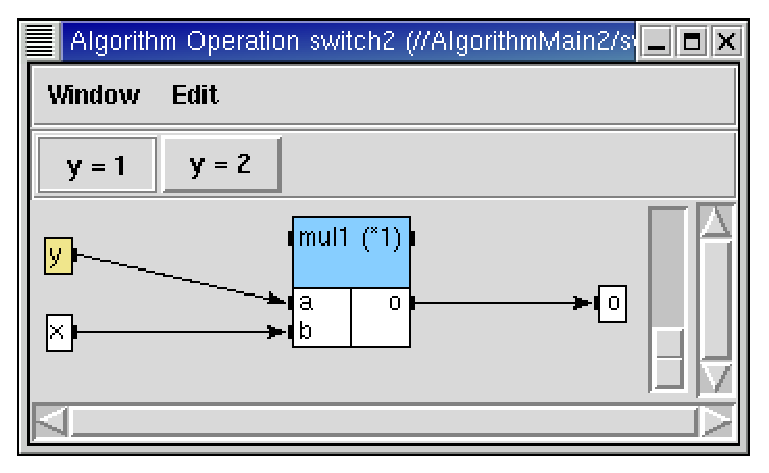
\includegraphics[width=0.48\linewidth]{Condition1_algo2.eps} 
  \end{center}
  \caption{Condition y=1}
  \label{condition1_algo2}
\end{figure}

\item click on the condition ``y=2'' (figure \ref{condition2_algo2}). 

and create the reference ``switch1'' (type \textbf{switch1}).

\begin{figure}[ht]
  \begin{center} 
        \includegraphics[width=0.48\linewidth]{Condition2_algo2.eps} 
  \end{center}
  \caption{Condition y=2}
  \label{condition2_algo2}
\end{figure}

\end{itemize}

\item Create dependences between the references.
\end{itemize}
The algorithm looks like the figure \ref{algo5_2}.

\begin{figure}[ht]
  \begin{center} 
        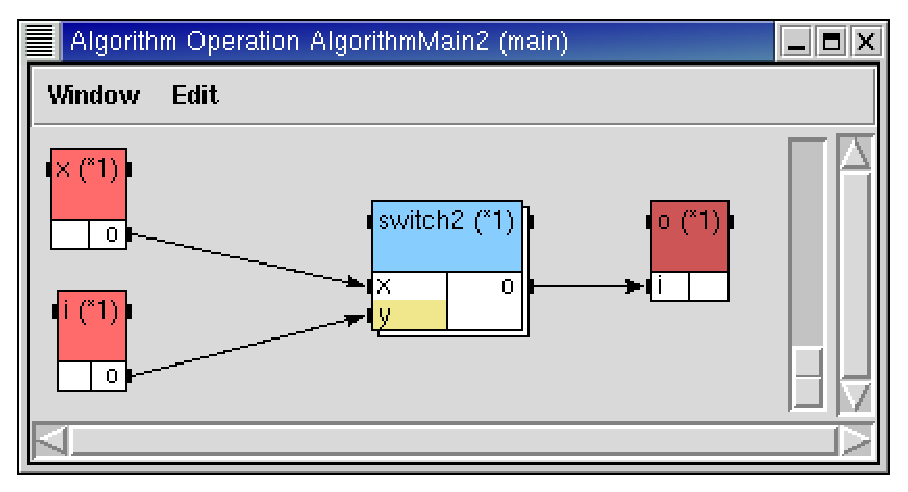
\includegraphics[width=0.52\linewidth]{algorithmMain2_ex5.eps} 
  \end{center}
  \caption{algorithm of the example 5}
  \label{algo5_2}
\end{figure}

\chapter{Example 6 : algorithm, architecture, adequation
and code generation}
\section{Creation of the algorithm}
Create an algorithm \textbf{algo} which looks like the figure \ref{algo6},
using the library \textbf{int} for the operations ``In<1>'' (\textbf{input}),
``cste2<{2}>'' (\textbf{cst}), ``add<1>'' (\textbf{Arit\_add}), ``mul<1>''
(\textbf{Arit\_mul}), ``visuadd<1>'' and ``visumul<1>'' (\textbf{output}). For the
operation ``conv'', create a function definition called \textbf{conv} and add
a reference to this definition. Create the dependences between the references.

\begin{figure}[htbp]
  \begin{center} 
        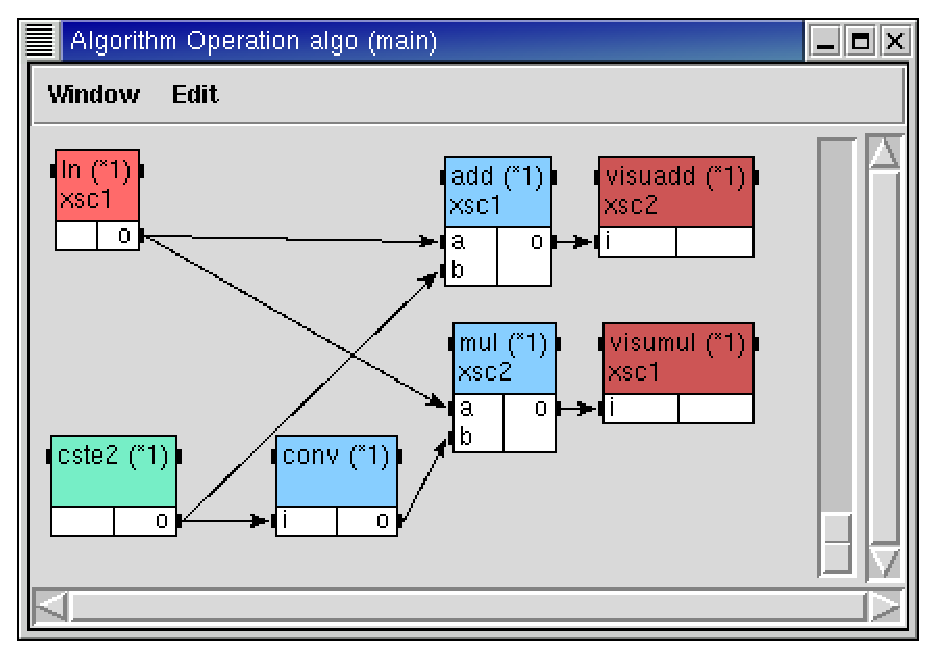
\includegraphics[width=0.52\linewidth]{algorithm_ex6.eps} 
  \end{center}
  \caption{algorithm of the example 6}
  \label{algo6}
\end{figure}

\section{Creation of the architecture}
\begin{itemize}
\item Using the library \textbf{U}, create two operators, ``pc1'' and the main
operator ``root'', and create a \textbf{communication media} with the name
``ppl''.

\item Create the connections between the operators and the media in the main
architecture ``archi''

The architecture looks like the figure \ref{archi6}.

\begin{figure}[htbp]
  \begin{center} 
        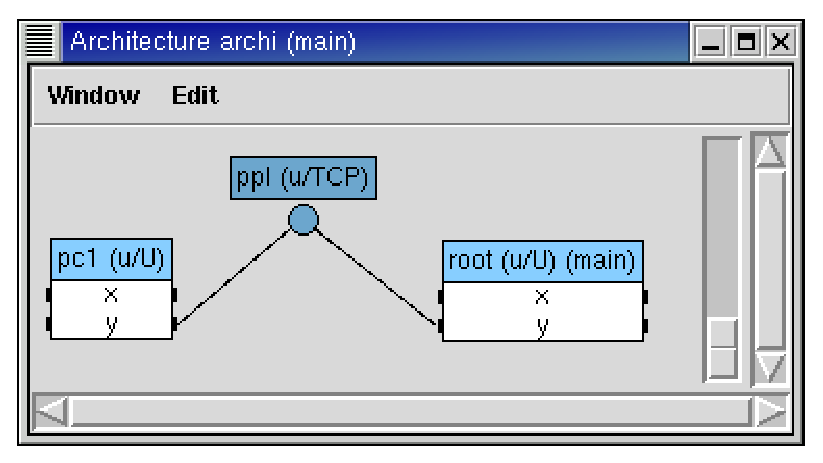
\includegraphics[width=0.48\linewidth]{architecture_ex6.eps} 
  \end{center}
  \caption{architecture of the example 6}
  \label{archi6}
\end{figure}

\item Create the Software Component \textbf{xsc1} and \textbf{xsc2} and create
the absolute constraints on the operators: \textbf{xsc1} on ``root'',
\textbf{xsc2} on ``pc1''.

Attach software component on the operations: 

``In'', ``add'' and ``visumul'' $\rightarrow$ \textbf{xsc1},

``mul'' and ``visuadd'' $\rightarrow$ \textbf{xsc2}.

\end{itemize}

\section{The Code Generation}
\begin{itemize}
\item Before performing the Code Generation, you have to perform the
  Adequation. In the principal window, Menu: \textbf{Adequation / Flatten} or F4

\item In the principal window,

Menu: \textbf{Code / Generate Code} (or F5).

This generate for each operator of the main architecture the code in a
file and an architecture description (file exemple.m4). These files are
generated in the same directory as the application. The files generated for
each processors may be viewed: 

Menu: \textbf{Code / View Code} (or F6). 

\item The macros corresponding to the operations, included in the libraries of
SynDEx are already defined in the folder ``macros''.

\item In the same folder as the SynDEx application of the example 6, create
a new file \textbf{example6.m4x} in which you define the macro corresponding to
the operation
\textbf{conv} which is the only one not defined in the library, and the number of iterations. The file looks like the figure
\ref{example6_m4x}.

\begin{figure}[hbtp]
\sf{\bf{
dnl (c)INRIA 2001\\
dnl SynDEx v6 executive macros specific to application example6.sdx\\
divert(-1)\\

\# ----------\\
\# NOTRACEDEF, when defined, prevents SynDEx macros from generating a
comment,\\
\# trace of the macro call, before the body of the generated code\\

define(`NOTRACEDEF')\\

define(`NBITERATIONS',5)\\

define(`conv',`ifelse(\\
MGC,`INIT',`dnl',\\
MGC,`LOOP',`\$2[0] = \$1[0] + 1;',\\
MGC,`END',`dnl')')\\

\# The following `divert' stops the output-discarding effect of the previous\\
\# `divert(-1)' at the top of this file, so this `\#include' is output from
m4:\\ 
divert\\ 
\#include <stdio.h> /* for printf */\\ 
divert(-1)\\
divert`'dnl---------------- end of file ------------------\\ 
}}
\label{example6_m4x}
\caption{\rm{the file example6.m4x}}
\end{figure}

\item Create a new file \textbf{example6.m4m}, in which you set for each
operator, except the main operator, the name of a workstation corresponding to
this operator.

The file looks like the figure \ref{example6_m4m}.

\begin{figure}[hbtp]
\sf{\bf{
dnl (c)INRIA 2001\\
dnl\\
dnl make specific macros: internet hostnames of processors\\
dnl\\
dnl root\_hostname\_ is substituted by default by the current host
name:\\
dnl                you do not need to, and should not, redefine 
it.\\
dnl p\_hostname\_ must be substituted by the name of a workstation
 granting rsh\\
dnl             requests from root\_hostname\_; it is substituted 
by default\\
dnl             simply by `p'; redefine it if needed.\\
define(`pc1\_hostname\_', charpentier)dnl\\
}}
\caption{\rm{the file example6.m4m}}
\label{example6_m4m}
\end{figure}

\item Create a new file \textbf{root.m4x} including the file
example6.m4m. The figure looks like the figure \ref{root_m4x}.

\begin{figure}[hbtp]
\sf{\bf{
dnl (c)INRIA 2001\\
dnl A symbolic link would be better, but Win95 does not support 
symbolic links.\\
include(example6.m4m)\\
}}
\caption{\rm{the file root.m4x}}
\label{root_m4x}
\end{figure}

\item Create a new file \textbf{GNUmakefile} which allows the compilation and
the substitution of the macros from the code generation by the executable code.

The file looks like the figure \ref{GNUmakefile} 
\begin{figure}[hbtp]
        \sf{\bf{
\# (c)INRIA 2001\\
\# WARNING: this file must be processed by GNU make (REQUIRED!)\\
\# SynDEx v6 main makefile for compiling SynDEx-generated executives,\\
\# example6.sdx application, bi-workstation target\\

\# Beginners: please start your reading with the README file.\\

\# \$(A) should be the application name\\
\# \$(M4) must be the GNU version of m4:\\
\# \$(M4PATH) must be the path to the *.m4? files defining SynDEx macros\\

A  = example6\\
M4 = gm4\\

export Macros\_Path = ../../../macros/Unix\_C\_TCP\\
export Libraries\_Path = ../../../macros/libraries\\
export M4PATH = \$(Macros\_Path):\$(Libraries\_Path)\\

CFLAGS = -DDEBUG\\

\# \$(VPATH) is searched by make for dependent files not found in \$(PWD)\\
VPATH = \$(M4PATH)\\

\# \$(A).sdx   is the SynDEx user-specification of the application\\
\# \$(A).m4    is the SynDEx-generated architecture file\\
\# xxx.m4     is the SynDEx-generated generic executive for processor xxx\\
\# syndex.m4m defines generic macros for generating makefiles\\
\# <type>.m4m contains compilation rules specific to processor type <type>\\
\# \$(A).mk    is the makefile generated from \$(A).m4\\
\# syndex.m4x defines generic macros for generating executives\\
\# <type>.m4x defines executive macros specific to processor type <type>\\
\# \$(A).m4x   contains user-defined executive macros specific to \$(A)\\
\# xxx.src    is the executive generated from xxx.m4 into the src language\\
\# \$(xxx.libs) application specific src/obj/libs to be linked to xxx.src\\
\# xxx       is the executable compiled from xxx.src (\_root is the launcher)\\

.PHONY: all clean\\
all : \$(A).mk \$(A).run\\
clean ::\\
        \$(RM) \$(A).mk *~ *.o *.a\\

\$(A).mk : \$(A).m4 syndex.m4m U.m4m \$(A).m4m\\
        \$(M4) \$< >\$@\\

root.libs = \\
p.libs = \\

include \$(A).mk\\
}}
        \caption{\rm{the file GNUmakefile}}
        \label{GNUmakefile}
\end{figure}

\end{itemize}

\newpage
The folder of the example 6 must contain the following files:
\begin{itemize}
\item example6.sdx
\item example6.m4
\item root.m4
\item pc1.m4
\item example6.m4x
\item example6.m4m
\item root.m4x
\item GNUmakefile
\end{itemize}

To launch the execution, type the command \textbf{gmake} in the folder of the
example 6. 

To delete the file created during the compilation, type the command
\textbf{gmake clean}.

\end{document}
